%\begin{frame}
%\frametitle{Interprétation statistique}
%\begin{maliste}
%\begin{center}
%\fbox{
%\parbox{0.8\linewidth}{
%\textcolor{blue}{
%$\mup$ = plus grande valeur de $\mu$ 
%pour laquelle observation et prévision en accord
%}
%}
%}
%\end{center}
%\vspace*{0.3cm}
%\item Calcul limite nécessite : 
%\begin{enumerate}
%\item Modèle statistique $P(\text{observation}|\mu)$
%\item Mesure quantitative de l'accord entre observation et prévision
%\item Niveau de confiance $1-\alpha$
%\end{enumerate}
%\end{maliste}
%\end{frame}

\begin{frame}
\frametitle{Interpr\'etation statistique}
%{Modèle statistique et inférences}

\begin{small}
\begin{maliste}
\item 2 interprétations : observation, exclusion
\vspace*{0.1cm}
\item Exclusion : limite sur section efficace (ou $\mu=\sigma/\sigma_\text{ref}$) $\rightarrow$ limites sur paramètres
\end{maliste}

\begin{center}
\fbox{
\parbox{0.8\linewidth}{
\textcolor{blue}{
$\mup$ = plus grande valeur de $\mu$ 
pour laquelle observation et prédiction sont en accord
}
}
}
\end{center}
\end{small}

\vspace*{-0.1cm}
\pause
\begin{varblock}[1.05\textwidth]{Modèle statistique}

\vspace*{-0.2cm}
\begin{columns}
\begin{column}{0.5\textwidth}
\begin{footnotesize}
\[
\hspace*{0.3cm}
P\left(\{\nc\}|\textcolor{blue}{\mu},\textcolor{red}{\{\scc,\bc\}}\right)=\prod\limits_c\frac{\left(\textcolor{blue}{\mu} \textcolor{red}{\scc}+\textcolor{red}{\bc}\right)^{\nc}}{\nc!}e^{-\left(\textcolor{blue}{\mu} \textcolor{red}{\scc}+\textcolor{red}{\bc}\right)}
\]
\end{footnotesize}
\end{column}

\begin{column}{0.5\textwidth}
\begin{maliste}
\item Nombreuses sources d'incertitudes
\vspace*{0.2cm}
\item $\nu_j$ : paramètres de nuisance 
$\rightarrow \textcolor{red}{\scc\left(\{\nu_j\}\right), \bc\left(\{\nu_j\}\right)}$
%\vspace*{0.2cm}
%\item $P\left(\{\nc\}|\textcolor{blue}{\mu},\textcolor{red}{\{\scc,\bc\}}\right)\rightarrow P\left(\{\nc\}|\textcolor{blue}{\mu},\textcolor{red}{\nu}\right)$
\end{maliste}
\end{column}
\end{columns}
\end{varblock}

\vspace*{-0.1cm}
\pause
\begin{block}{Approches d'inférence}
\begin{columns}
\begin{column}{0.65\textwidth}
\begin{maliste}
\item 3 approches : bayésienne, fréquentiste, hybride
\vspace*{0.1cm}
\item Variantes : $\CLs$, PCL, test statistique classique vs profilé, priors subjectifs vs objectifs, etc.
\end{maliste}
\end{column}
\begin{column}{0.35\textwidth}
\[
\hspace*{-1cm}
P\left(\{\nc\}|\textcolor{blue}{\mu},\textcolor{red}{\nu}\right)\rightarrow P\left(\{\nc\}|\textcolor{blue}{\mu}\right)\]
\end{column}
\end{columns}
\end{block}

\end{frame}

\begin{frame}
\frametitle{Approches bayésienne, fréquentiste et hybride : généralités}
\begin{block}{Approche bayésienne}
\begin{columns}
\begin{column}{0.6\textwidth}
\begin{maliste}
\item Distribution \posterior~du paramètre d'intérêt :
\[f\left(\mu|\{\nc\}\right)\propto \displaystyle\int P\left(\{\nc\}|\textcolor{blue}{\mu},\textcolor{red}{\nu}\right)\underbrace{\pi_\nu\left(\nu\right)\pi_\mu\left(\mu\right)}_{priors}\dd\textcolor{red}{\nu}\]
%\item Limite d'exclusion :
%\[\displaystyle\int_{0}^{\mup} f\left(\mu|\{\nc\}\right)\dd\mu=1-\alpha\]
\end{maliste}
\end{column}
\begin{column}{0.4\textwidth}
\begin{center}
\vspace*{-0.3cm}
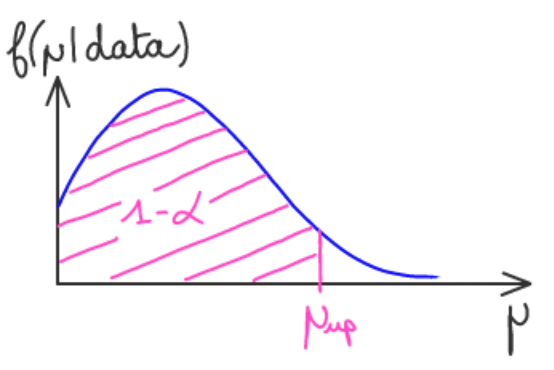
\includegraphics[width=0.7\textwidth]{Figures/Stat/posteriorIllustration.png}
\end{center}
\end{column}
\end{columns}
\end{block}


\begin{varblock}[1.05\textwidth]{Approche fréquentiste et hybride}
\begin{columns}
\begin{column}{0.6\textwidth}
\begin{maliste}
\item Test d'hypothèse classique
\begin{itemize}
\item Variable de test : $\qmu=\qmu(\{\nc\},\nu)$
\item Construction Neyman unilatérale
\end{itemize}
\item Méthode \CLs{} :
\[\pval \rightarrow \CLs=\frac{P\left(\qmu<\qmuobs|H_0\right)}{P\left(\qmu<\qmuobs|H_1\right)}\]
\item \pval{} : $p\left(\mu,\nu\right)$
\end{maliste}
\end{column}
\begin{column}{0.4\textwidth}
\begin{center}
\vspace*{-0.7cm}
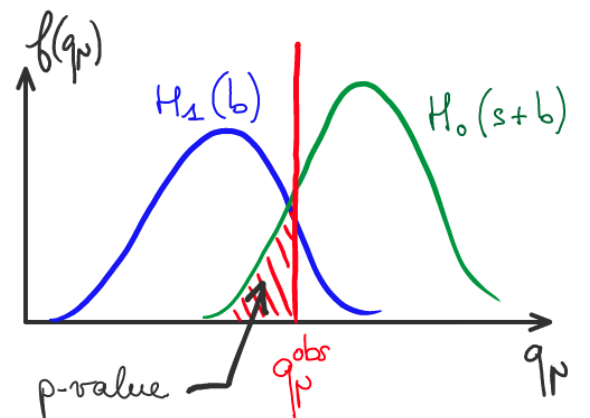
\includegraphics[width=0.7\textwidth]{Figures/Stat/pValueIllustration_cropped.png}
\end{center}
\begin{center}
\vspace*{-0.2cm}
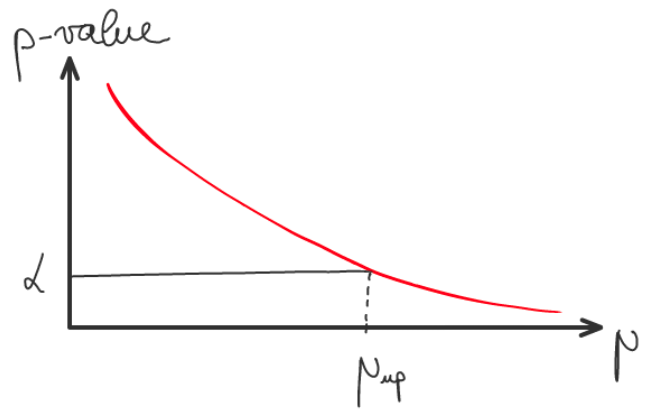
\includegraphics[width=0.7\textwidth]{Figures/Stat/NeymanConstruction1D_cropped.png}
\end{center}
\end{column}
\end{columns}
\end{varblock}
\end{frame}

%\begin{frame}
%\frametitle{Approches fréquentiste et hybride}
%\begin{columns}
%\begin{column}{0.7\textwidth}
%\begin{maliste}
%\item Test d'hypothèse classique
%\begin{itemize}
%\item Variable de test : $\qmu=\qmu(\{\nc\},\nu)$ 
%\item Construction Neyman unilatérale
%\item Méthode \CLs{} : 
%\[\pval \rightarrow \CLs=\frac{P\left(\qmu<\qmuobs|H_0\right)}{P\left(\qmu<\qmuobs|H_1\right)}\]
%\end{itemize}
%\end{maliste}
%\end{column}
%\begin{column}{0.4\textwidth}
%\begin{center}
%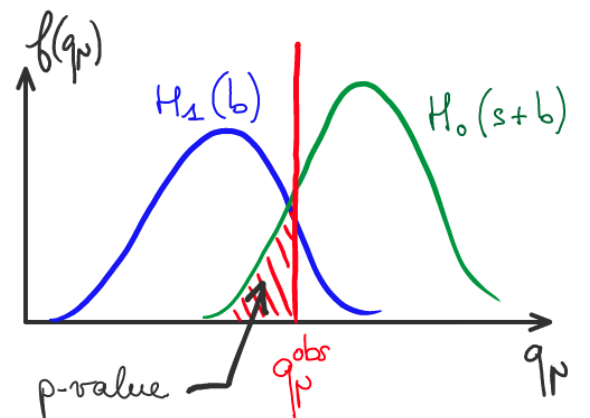
\includegraphics[width=1\textwidth]{Figures/Stat/pValueIllustration_cropped.png}
%\end{center}
%\end{column}
%\end{columns}
%\pause
%\begin{columns}
%\begin{column}{0.5\textwidth}
%\begin{center}
%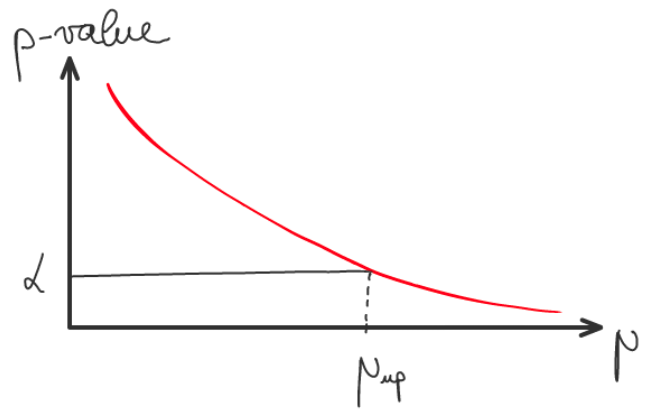
\includegraphics[width=1\textwidth]{Figures/Stat/NeymanConstruction1D_cropped.png}
%\end{center}
%\end{column}
%\begin{column}{0.5\textwidth}
%\begin{maliste}
%\item \pval{} : $p\left(\mu,\nu\right)$
%\item Diff. fréquentiste/hybride~: traitement des incertitudes
%\end{maliste}
%\end{column}
%\end{columns}
%\end{frame}

\begin{frame}
\frametitle{Approche hybride}

\begin{small}

\begin{maliste}
\item Origine : Cousins-Highland NIM A320 (1992) 331-335
\vspace*{0.1cm}
\item Test d'hypothèse basé sur vraisemblance marginalis\'ee
\[
%\hspace*{-0.5cm}
\begin{split}
P\left(\{\nc\}|\textcolor{blue}{\mu}\right)&= \Ewrt{\nu}{P\left(\{\nc\}|\textcolor{blue}{\mu},\textcolor{red}{\nu}\right)}\\
&=
\displaystyle\int
P\left(\{\nc\}|\textcolor{blue}{\mu},\textcolor{red}{\nu}\right)\times\prod_j\underbrace{\pi_j\left(\textcolor{red}{\nu_j}\right)}_{priors}\dd\textcolor{red}{\nu_j} 
\end{split}
\]

%\pause

\vspace*{-0.8cm}
\begin{columns}
\begin{column}{0.5\textwidth}
\begin{center}
%\hspace*{-1cm}
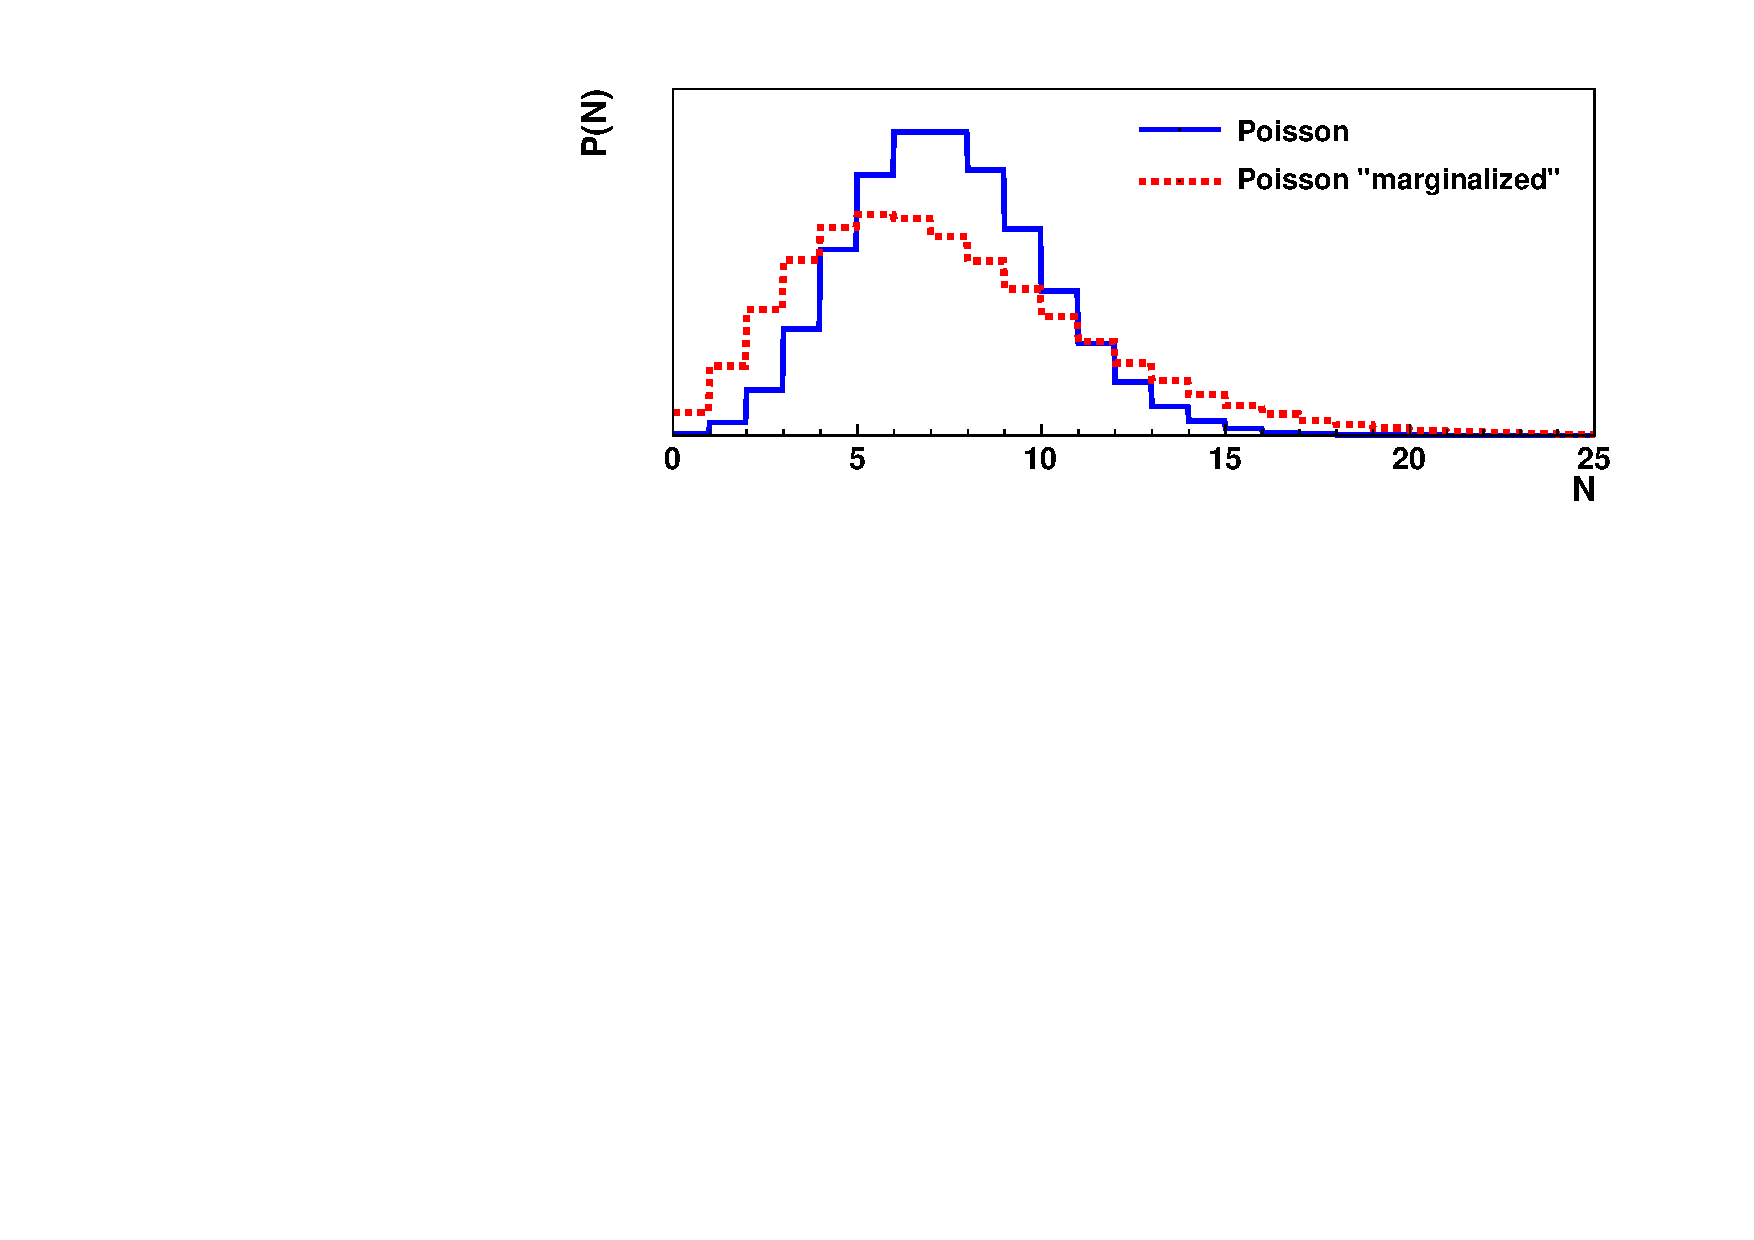
\includegraphics[width=1.2\textwidth]{Figures/Stat/PoissonGammaCompoundExample_compound.pdf}
\end{center}
\end{column}
\begin{column}{0.5\textwidth}
\begin{center}
\vspace*{0.4cm}
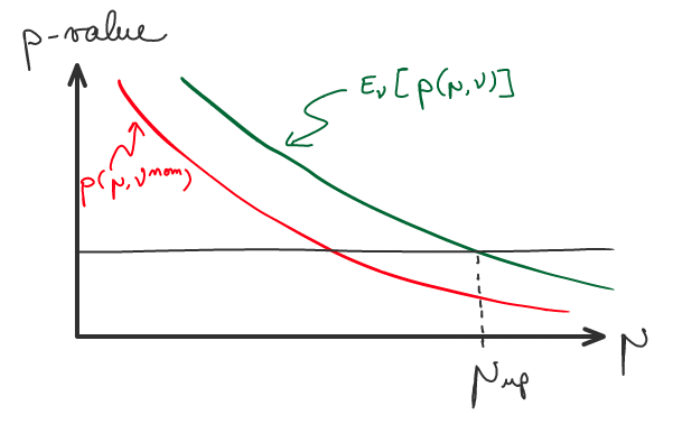
\includegraphics[width=0.9\textwidth]{Figures/Stat/NeymanConstruction1DHybrid_cropped.png}
\end{center}
\end{column}
\end{columns}

%\pause 
\end{maliste}
\vspace*{-0.2cm}

\begin{block}{\'Equivalence Hybride - Bay\'esien (arXiv:1404.1340)}
\textcolor{magenta}{Hybride~(\CLs) = bayésien (\english{prior} uniforme) si : $\bullet$ une seule observable}
\textcolor{magenta}{\phantom{Hybride~(\CLs) = bayésien (\english{prior} uniforme) si :} $\bullet$ aucune incertitude sur signal}
\textcolor{magenta}{\phantom{Hybride~(\CLs) = bayésien (\english{prior} uniforme) si :} $\bullet$ niveau cr\'edibilit\'e = niveau confiance}
\end{block}
\end{small}

\end{frame}

\begin{frame}
\frametitle{Approche fréquentiste}
\begin{small}

\begin{columns}
\begin{column}{0.6\textwidth}
%\begin{maliste}
%\item Mod\`ele statistique :
%\end{maliste}
\qquad Mod\`ele statistique complet :
\end{column}
\begin{column}{0.5\textwidth}
\end{column}
\end{columns}

\begin{block}{}
\[
\hspace*{-0.5cm}
P(\{\nc\},\{a_j\}|\textcolor{blue}{\mu},\textcolor{red}{\nu})=\underbrace{\prod\limits_c\frac{\left(\textcolor{blue}{\mu} \scc(\textcolor{red}{\nu_j})+\bc(\textcolor{red}{\nu_j})\right)^{\nc}}{\nc!}e^{-\left(\textcolor{blue}{\mu} \scc(\textcolor{red}{\nu_j})+\bc(\textcolor{red}{\nu_j})\right)}}_{\text{expérience principale}}\underbrace{\prod_j P_j\left(a_j|\textcolor{red}{\nu_j}\right)}_{\text{expériences auxilliaires}}\]
\end{block}
\end{small}

%\pause
\begin{small}
\begin{columns}
\begin{column}{0.6\textwidth}
\begin{maliste}
\item Variable de test : vraisemblance profilée
\begin{footnotesize}
\[
\hspace*{-0.3cm}
\qmu=\left\{
\begin{tabular}{c l}
$-2\ln\displaystyle\frac{P(\{\nc\},\{a_j\}|\textcolor{blue}{\mu},\textcolor{red}{\EstCond{\nu}})}{P\left(\{\nc\},\{a_j\}|\textcolor{blue}{\Est{\mu}},\textcolor{red}{\Est{\nu}}\right)}$ & \text{si $\mu\geq\Est{\mu}$} \\
$0$ & \text{si $\mu < \Est{\mu}$}.
\end{tabular}
\right.
\]
\end{footnotesize}
\item Construction Neyman complète impossible
\begin{itemize}
\item[$\rightarrow$] Hybrid resampling method : $\nu^\text{sup}\simeq\EstCond{\nu}(\mu)$
%\item[$\rightarrow$] Ok dans limite asymptotique
\end{itemize}
\end{maliste}
\end{column}
\begin{column}{0.5\textwidth}
\begin{center}
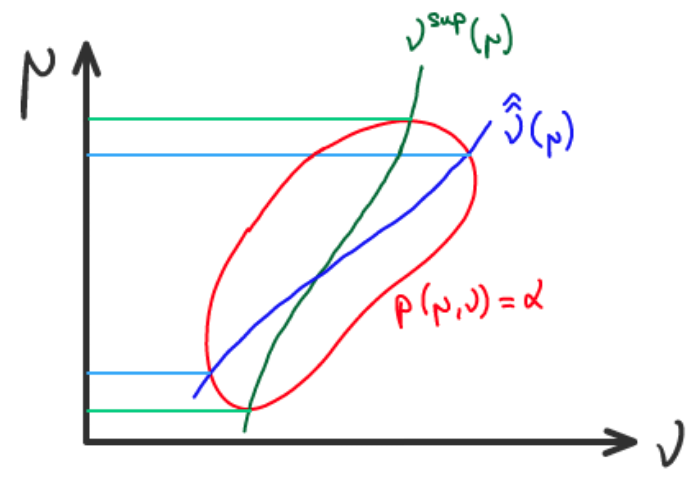
\includegraphics[width=0.9\textwidth]{Figures/Stat/FullNeymanConstructionWithApprox_cropped}
\end{center}
\end{column}
\end{columns}

\begin{columns}
\begin{column}{0.6\textwidth}
\begin{maliste}
\item Limite asymptotique (Wald, 1943) :
\end{maliste}
\end{column}
\begin{column}{0.5\textwidth}
\end{column}
\end{columns}

%\vspace*{-0.1cm}
\[-2\ln\displaystyle
\frac{P(\{\nc\},\{a_j\}|\textcolor{blue}{\mu},\textcolor{red}{\EstCond{\nu}})}{P\left(\{\nc\},\{a_j\}|\textcolor{blue}{\Est{\mu}},\textcolor{red}{\Est{\nu}}\right)} 
\tendsto{n}{\infty} \displaystyle\frac{\left(\mu-\Est{\mu}\right)^2}{\sigma^2}\]


\end{small}

\end{frame}

%\begin{maliste}
%\item $\mu$ rejeté ssi $p\left(\mu,\nu\right)<\alpha,~\forall\nu$ 
%\vspace*{0.2cm}
%\item $\nu^\text{sup}$=valeur qui maximise $p\left(\mu,\nu\right)$\\
%$\rightarrow$ $\mu$ rejeté ssi $p\left(\mu,\nu^\text{sup}\right)<\alpha$
%\vspace*{0.2cm}
%\item Approximation :
%\[\nu^\text{sup}\simeq\EstCond{\nu}(\mu)\]

\begin{comment}
\begin{frame}
\frametitle{Approche fréquentiste : limite asymptotique}
\begin{small}
\hspace*{-4cm}
\begin{maliste}
\item Vraisemblance profil\'ee dans limite asymptotique (Wald, 1943) :
\end{maliste}

\[-2\ln\displaystyle
\frac{P(\{\nc\},\{a_j\}|\textcolor{blue}{\mu},\textcolor{red}{\EstCond{\nu}})}{P\left(\{\nc\},\{a_j\}|\textcolor{blue}{\Est{\mu}},\textcolor{red}{\Est{\nu}}\right)} 
\tendsto{n}{\infty} \displaystyle\frac{\left(\mu-\Est{\mu}\right)^2}{\sigma^2}\]

\vspace*{0.5cm}


\begin{columns}
\begin{column}{0.6\textwidth}
\begin{maliste}
\item Distribution $\qmu$ connue ($\chi^2$) \\
$\Rightarrow$ possible de calculer \pval s~analytiquement
\[\mup=\Est{\mu}+\sigma\Phi^{-1}\left[1-\alpha\times\Phi\left(\frac{\Est{\mu}}{\sigma}\right)\right]\]
%\item $\sigma$ ?
%\begin{itemize}
%\item Echantillon asymov $\mu' \rightarrow \Est{\mu}\simeq\mu'$   
%\end{itemize}
%\[\Rightarrow \qmuA\simeq\frac{\left(\mu-\mu'\right)^2}{\sigma^2}\]
\item Limite attendue à $N\sigma$ sous hyp. $\mu'$:
\[\Est{\mu}=\mu' + N\sigma\]
\end{maliste}
\end{column}
\begin{column}{0.5\textwidth}
\begin{center}
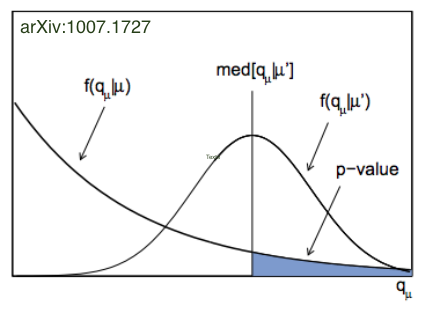
\includegraphics[width=1\textwidth]{Figures/Stat/PLRAsymptoticDistribs.png}
\end{center}
\end{column}
\end{columns}
\end{small}
\end{frame}
\end{comment}

%\begin{frame}
%\frametitle{Approche hybride et fréquentiste : limites attendues}
%\begin{maliste}
%\item Limites attendues :
%\fig{Distribution $\mup$}
%\end{maliste}
%\end{frame}

\begin{frame}
\frametitle{Aspects pratiques}
\begin{maliste}
\item Problème complexe :
\begin{itemize}
\item Plusieurs dizaines/centaines de paramètres de nuisance
\item Plusieurs bruits de fonds, canaux, distributions
\item Corrélations entre bruits de fond, canaux, bins
\vspace*{0.2cm}
\begin{center}
\textcolor{red}{$\rightarrow$ pas de solutions analytiques}
\end{center}
\end{itemize}
\vspace*{0.3cm}
\pause
\item Nécessité d'outils performants en terme de :
\begin{itemize}
\item Temps de calcul %(notamment pour optimisation sélection)
%dire que pour faire calculs rapides on est souvent oblige de faire approximations non souhaitables
\item Configurabilité 
\item Robustesse
\end{itemize}
\vspace*{0.3cm}
\pause
\item Outils \textcolor{blue}{utilisés}/\textcolor{magenta}{développés} :
\begin{itemize}
\item Hybride $\rightarrow$ \textcolor{blue}{\mclimit{}} et \textcolor{magenta}{\OTH}
\item Bayésien $\rightarrow$ \textcolor{magenta}{\tifosi}~(utilise \roofit{} et \roostats)
\item Fréquentiste $\rightarrow$ \textcolor{blue}{\histfactory+\roostats}
\end{itemize}
\end{maliste}
\end{frame}

\begin{comment}
\begin{frame}
\frametitle{Modèle statistique : \mclimit, \OTH{} et \tifosi}

\vspace*{-0.7cm}
\begin{small}
\[
\hspace*{-0.5cm}
P\left(\{\nc\}|\textcolor{blue}{\mu}\right)=\displaystyle\int P\left(\{\nc\}|\textcolor{blue}{\mu},\textcolor{red}{\{\scc',\bci',\eta_j\}}\right)\times \underbrace{\textcolor{red}{\prod\limits_{c}f\left(\scc'\right)\prod\limits_{i}f\left(\bci'\right)\prod\limits_{j}g\left(\eta_j\right)}}_{priors}\textcolor{red}{\dd\scc'\dd\bci'\dd\eta_j}
\]
\end{small}

\vspace*{-0.5cm}
\begin{columns}
\begin{column}{0.5\textwidth}
\begin{center}
%\vspace*{-0.3cm}
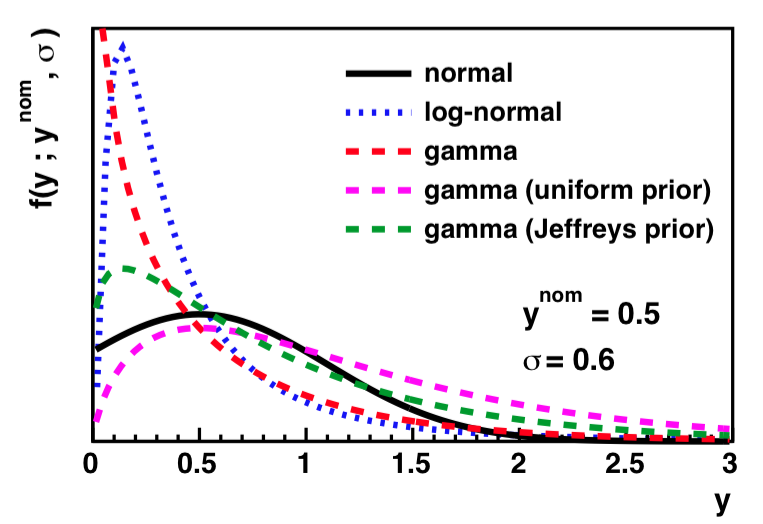
\includegraphics[width=0.78\textwidth]{Figures/Stat/plotNormalLogNGamma_cropped.png}
\end{center}
\end{column}
\begin{column}{0.5\textwidth}
%\vspace*{0.3cm}
\begin{center}
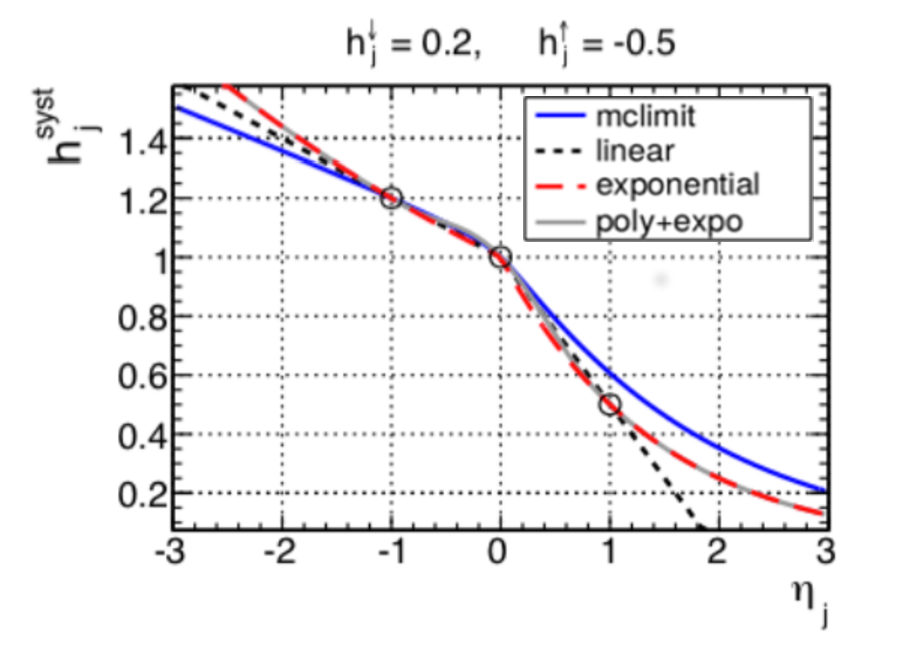
\includegraphics[width=0.82\textwidth]{Figures/Stat/cFunctionsInterExtrap_cropped3.pdf}
\end{center}
\end{column}
\end{columns}

\pause
\begin{center}
\vspace*{-0.3cm}
\hspace*{-1cm}
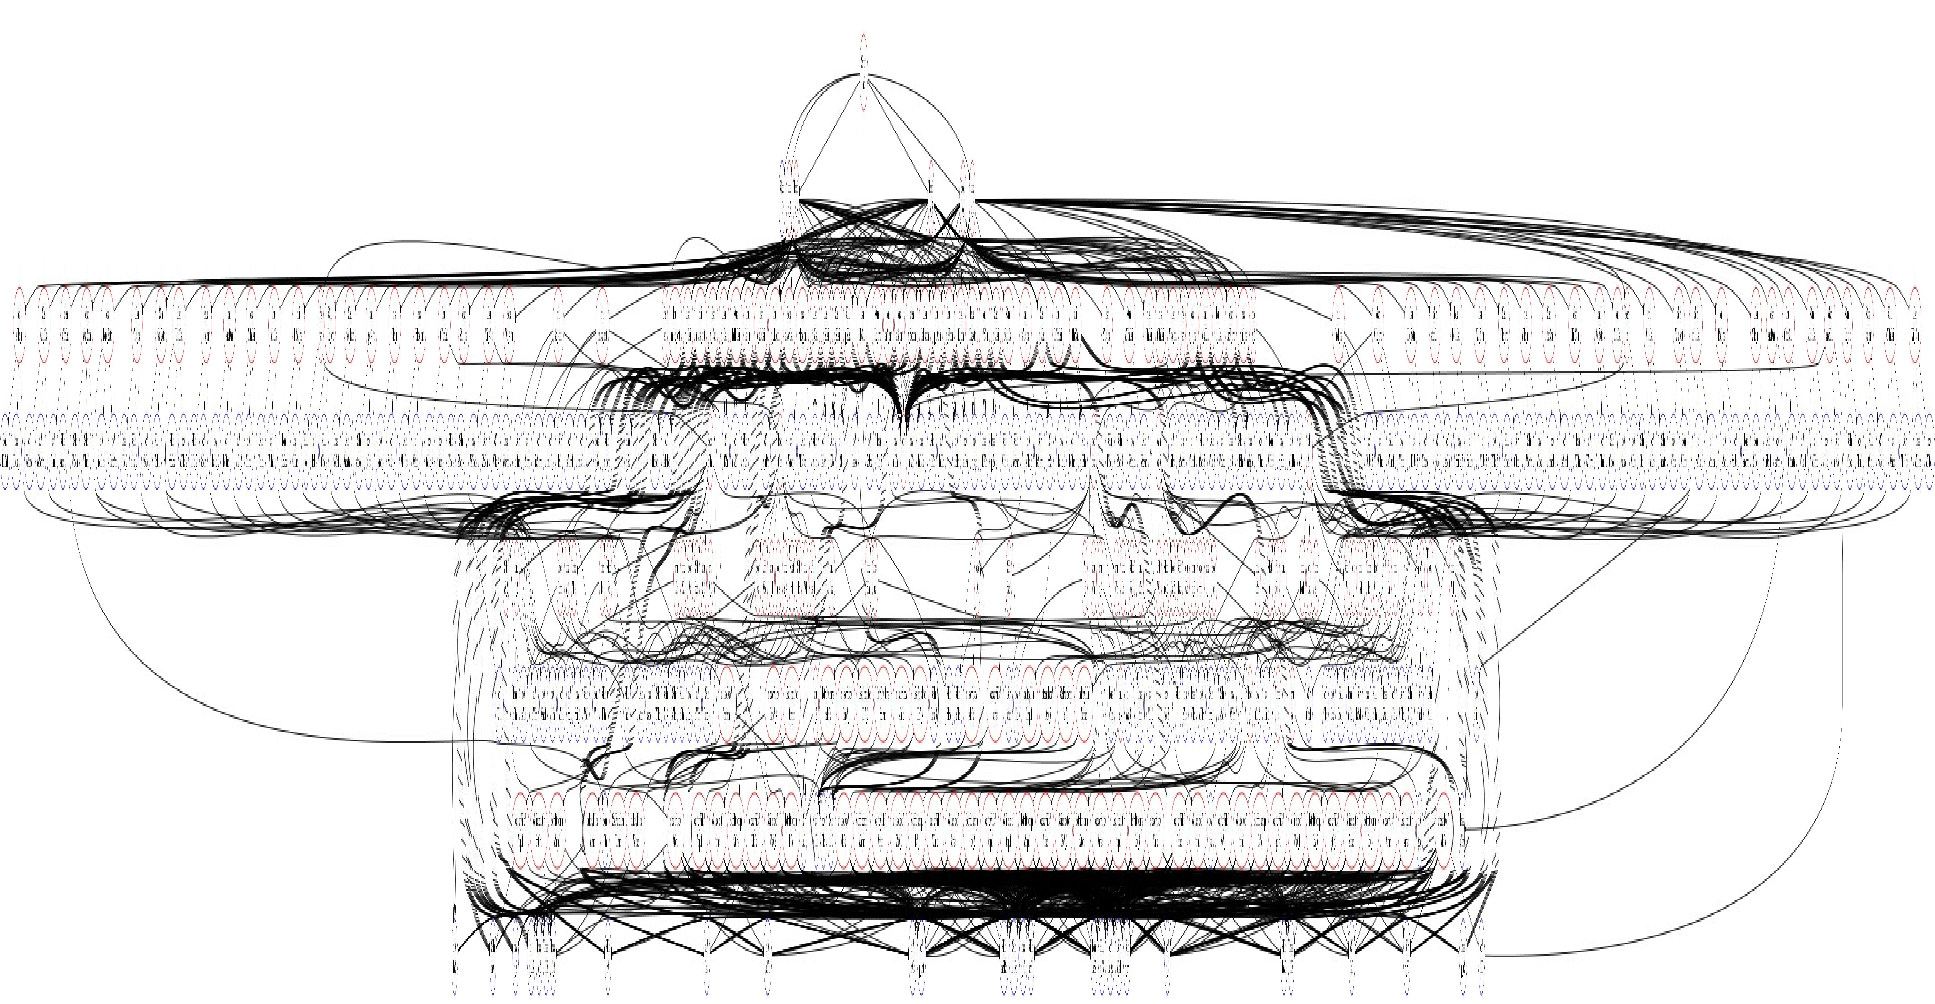
\includegraphics[width=13cm,height=3.5cm]{Figures/Stat/testGraphViz.pdf}
%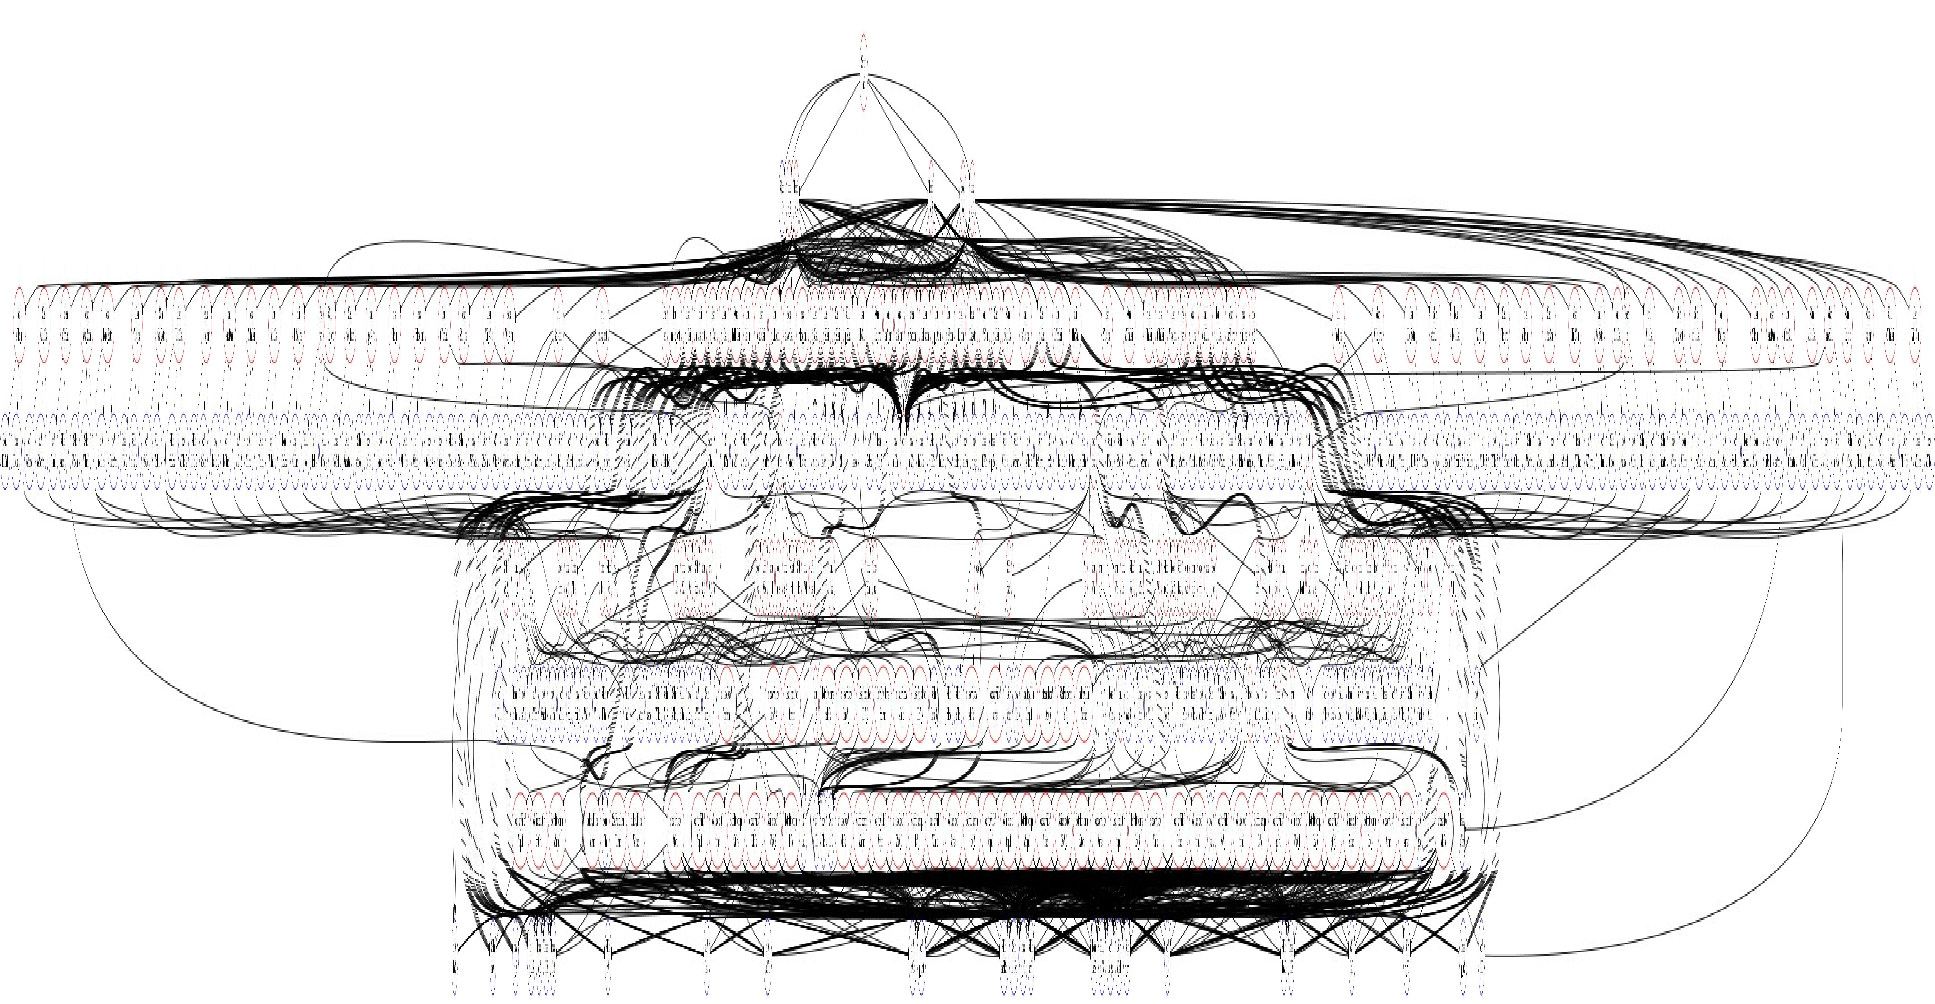
\includegraphics[scale=1]{Figures/Stat/testGraphViz.pdf}
\end{center}

%\begin{maliste}
%\item Pour chaque échantillon :
%\begin{itemize}
%\item Une incertitude statistique (taille finie échantillon) : 
%\begin{itemize}
%\item[$\rightarrow$] paramètre de nuisance : \textcolor{red}{$\scc'$}, \textcol%or{red}{$\bci'$}
%\item[$\rightarrow$] corrélation = 0\%
%\end{itemize}
%\vspace*{0.2cm}
%\item Une ou plusieurs incertitudes systématiques (sections efficaces, id, cali%brations, ...) 
%\begin{itemize}
%\item[$\rightarrow$] paramètres de nuisance : \textcolor{red}{$\eta_j$}
%\item[$\rightarrow$] corrélation = 0\% ou 100\%
%\end{itemize}
%\end{itemize}
%\end{maliste}

%\[\lhood(\textcolor{blue}{\mu},\textcolor{red}{\{\nu_j\}})\rightarrow\lhood(\textcolor{blue}{\mu},\textcolor{red}{\{\underbrace{\scc',\bci'}_{stat.},\underbrace{\eta_j}_{syst.}\}})\]

%\vspace*{-0.3cm}
%\begin{small}
%\begin{center}
%$\rightarrow$ 3 implémentations totalement indépendantes
%\item Choix interp/extrap et prior stat. \mclimit{}
%\item Ces choix sont pas top -> d'autres choix ont été implémentés dans \OTH{} et \tifosi
%\end{center}
%\end{small}


\end{frame}
\end{comment}

\begin{comment}
\begin{frame}
\frametitle{Incertitudes}

\vspace*{-0.3cm}

\begin{footnotesize}
\[
\hspace*{-0.5cm}
P\left(\{\nc\}|\textcolor{blue}{\mu}\right)=\displaystyle\int P\left(\{\nc\}|\textcolor{blue}{\mu},\textcolor{red}{\{\scc',\bci',\eta_j\}}\right)\times \textcolor{red}{\prod\limits_{c}f\left(\scc'\right)\prod\limits_{i}f\left(\bci'\right)\prod\limits_{j}g\left(\eta_j\right)}\textcolor{red}{\dd\scc'\dd\bci'\dd\eta_j}
\]
\end{footnotesize}

\vspace*{-0.2cm}
\begin{small}
\begin{varblock}[1.05\textwidth]{Incertitudes systématiques}
\vspace*{-0.3cm}
\begin{columns}
\begin{column}{0.6\textwidth}
\begin{maliste}
%\item Pour chaque source d'incertitude, on connait effet à $+1\sigma$ et $-1\sigma$. 
%\vspace*{0.2cm}
\item Exemples : x-sec, JES, b-tag, etc.
\item Param\`etres de nuisance : $\eta_j$
\item Interpolation pour $|\eta_j| \leq 1$
\item Extrapolation pour $|\eta_j| > 1$
\item Fonction interp./extrap. monotone par partie
%\begin{itemize}
%\item Interpolation entre $-1\sigma$, nominal et $+1\sigma$
%\item Extrapolation au-dela
%\item Monotone par partie
%\item Passe par les 3 points connus
%\end{itemize}
\end{maliste}
\end{column}
\begin{column}{0.4\textwidth}
\begin{center}
\vspace*{-0.5cm}
\hspace*{-0.5cm}
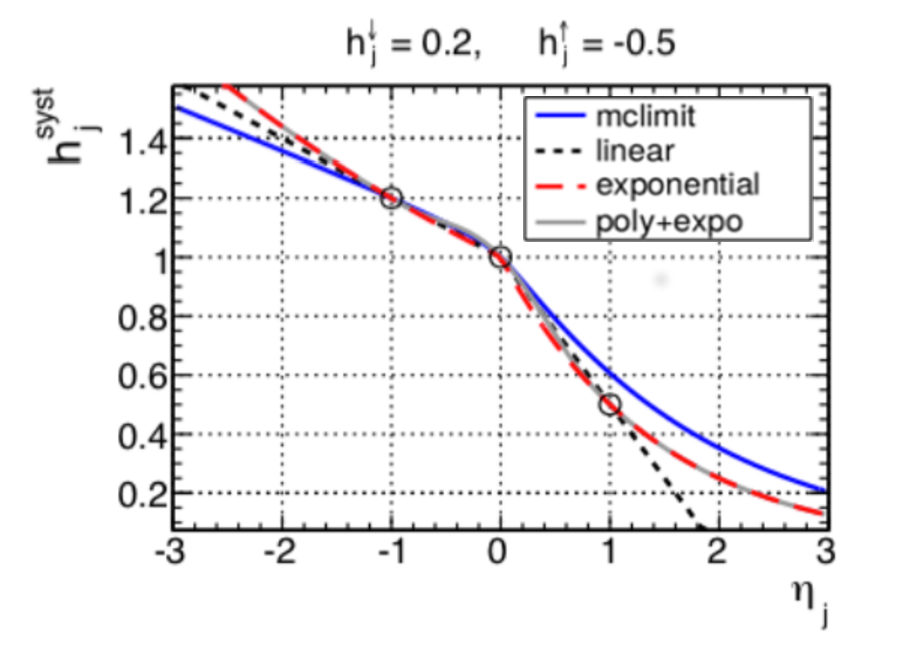
\includegraphics[width=0.9\textwidth]{Figures/Stat/cFunctionsInterExtrap_cropped3.pdf}
\end{center}
\end{column}
\end{columns}
\end{varblock}

\pause

\begin{varblock}[1.04\textwidth]{Incertitudes statistiques}
\begin{columns}

\begin{column}{0.4\textwidth}

\begin{center}
\vspace*{-0.5cm}
\hspace*{0.3cm}
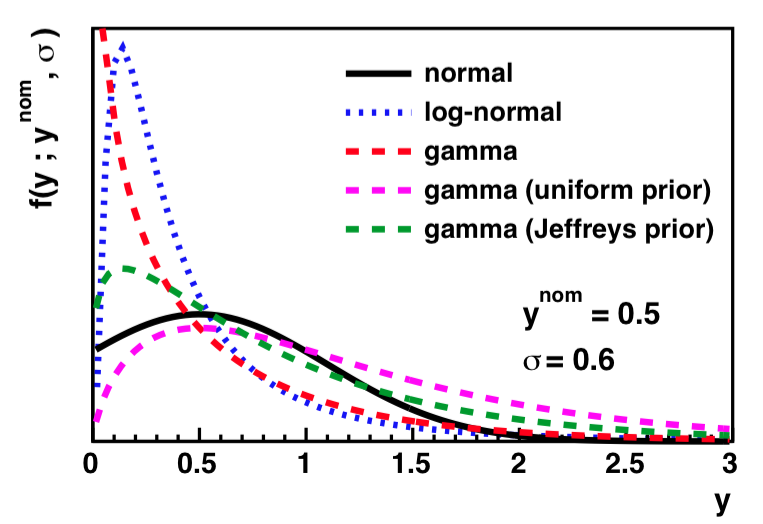
\includegraphics[width=0.9\textwidth]{Figures/Stat/plotNormalLogNGamma_cropped.png}
\end{center}
\end{column}
\begin{column}{0.6\textwidth}
\begin{maliste}
\vspace*{-0.2cm}
\item Param\`etres de nuisance : \textcolor{red}{\english{yield}} (\textcolor{red}{$y$}) ou \textcolor{red}{$\nu$}
\vspace*{-0.1cm}
\[\textcolor{red}{y} = \textcolor{red}{\nu}\times y^\text{nom}\]
\pause
\vspace*{-0.5cm}
\item Estimation \english{yield} = expérience poissonnienne
\vspace*{-0.1cm}
\[
\begin{small}
P(N_\text{aux};\textcolor{red}{\nu})=\frac{\left(\textcolor{red}{\nu} N_\text{aux}^\text{nom}\right)^{N_\text{aux}}}{\Gamma\left(N_\text{aux}+1\right)}e^{-\textcolor{red}{\nu} N_\text{aux}^\text{nom}}
\end{small}
\]
\vspace*{-0.3cm}
\item Distribution \posterior~de $\nu$
\[
\begin{small}
f\left(\textcolor{red}{\nu}\right|N_\text{aux}^{\text{nom}})\propto P(N_\text{aux}=N_\text{aux}^{\text{nom}};\textcolor{red}{\nu})\pi\left(\textcolor{red}{\nu}\right) 
\end{small}
\]
\end{maliste}
\end{column}

\end{columns}
\end{varblock}

\end{small}
\end{frame}
\end{comment}

\begin{frame}
\frametitle{\OTH}

\vspace*{-1cm}
\begin{columns}

\begin{column}{0.5\textwidth}
\vspace*{0.8cm}
\begin{block}{}
\begin{maliste}
\item Développé avec D. Calvet et T.~Thevenaux-Pelzer
\item arXiv:1502.02610
\item \begin{footnotesize}$\qmu=-2\ln\frac{\Lh\left(\mu,\nu_j=\nu_j^\text{nom}\right)}{\Lh\left(\mu=0,\nu_j=\nu_j^\text{nom}\right)}$\end{footnotesize}
\item Marginalisation $\rightarrow$ Intégration MC
\end{maliste}
\vspace*{-0.3cm}
\begin{figure}[!htb]
\begin{center}
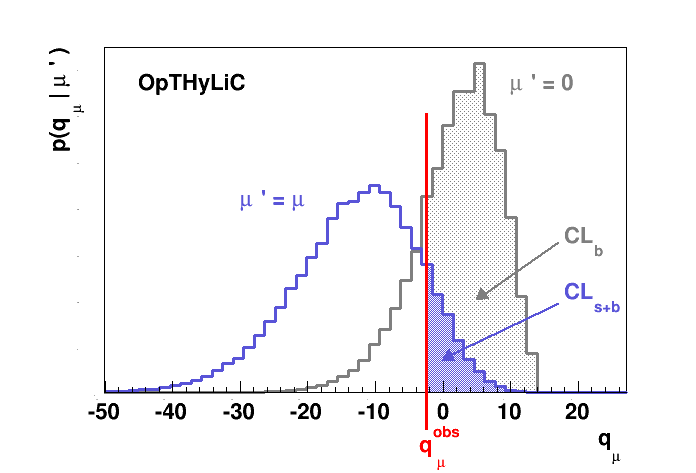
\includegraphics[width=0.8\textwidth]{Figures/Stat/testStatDistribExample.png}
\end{center}
\end{figure}
\begin{maliste}
\vspace*{-0.3cm}
\item Validation : comparaison avec
\begin{itemize}
\item Solutions analytiques
\item Solutions asymptotiques
\item \mclimit
\end{itemize}
\end{maliste}
\end{block}
\end{column}

\begin{column}{0.5\textwidth}
\begin{figure}[!htb]
\begin{center}
\pause
\vspace*{0.4cm}
\hspace*{0.3cm}
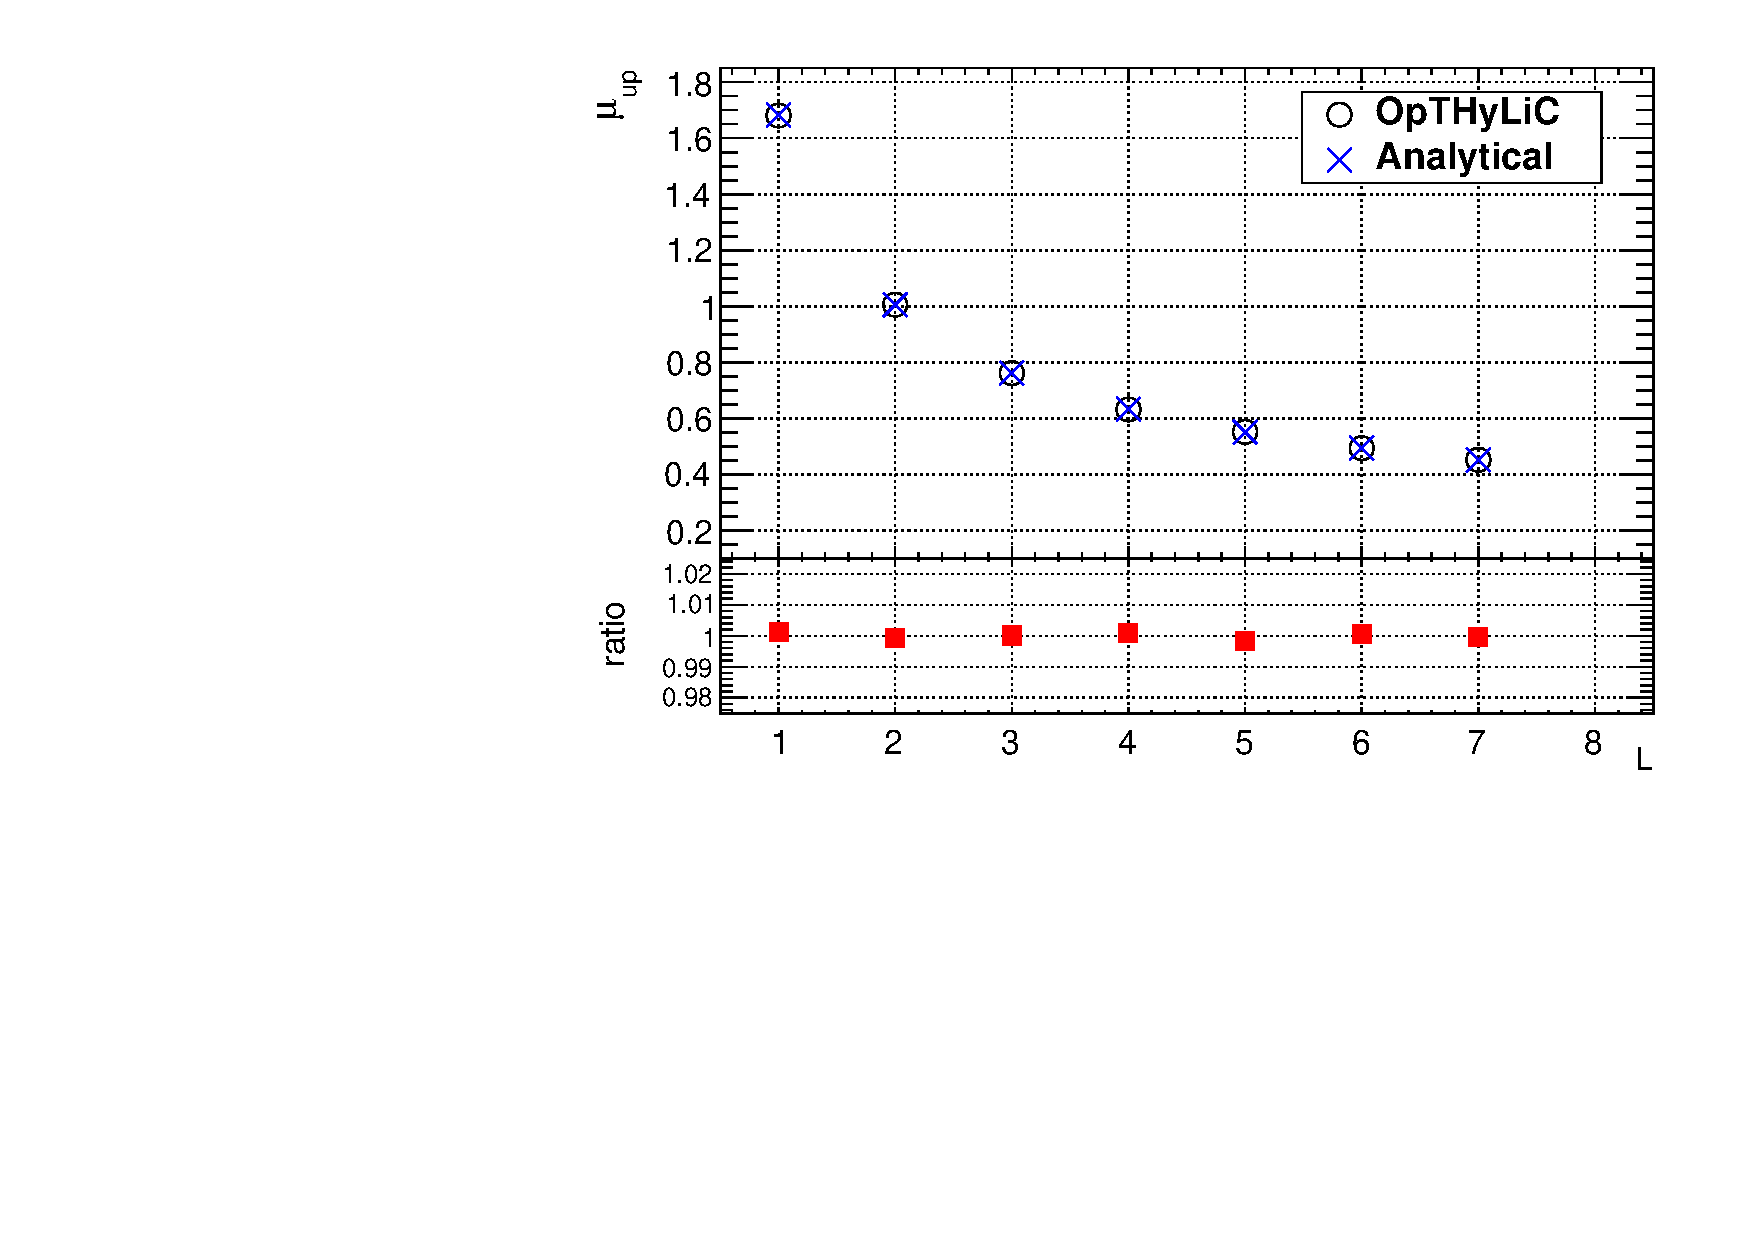
\includegraphics[width=1\textwidth]{Figures/Stat/SingleChannelNoUncertainties.pdf} \\
\pause
\vspace*{-0.8cm}
\hspace*{-0.5cm}
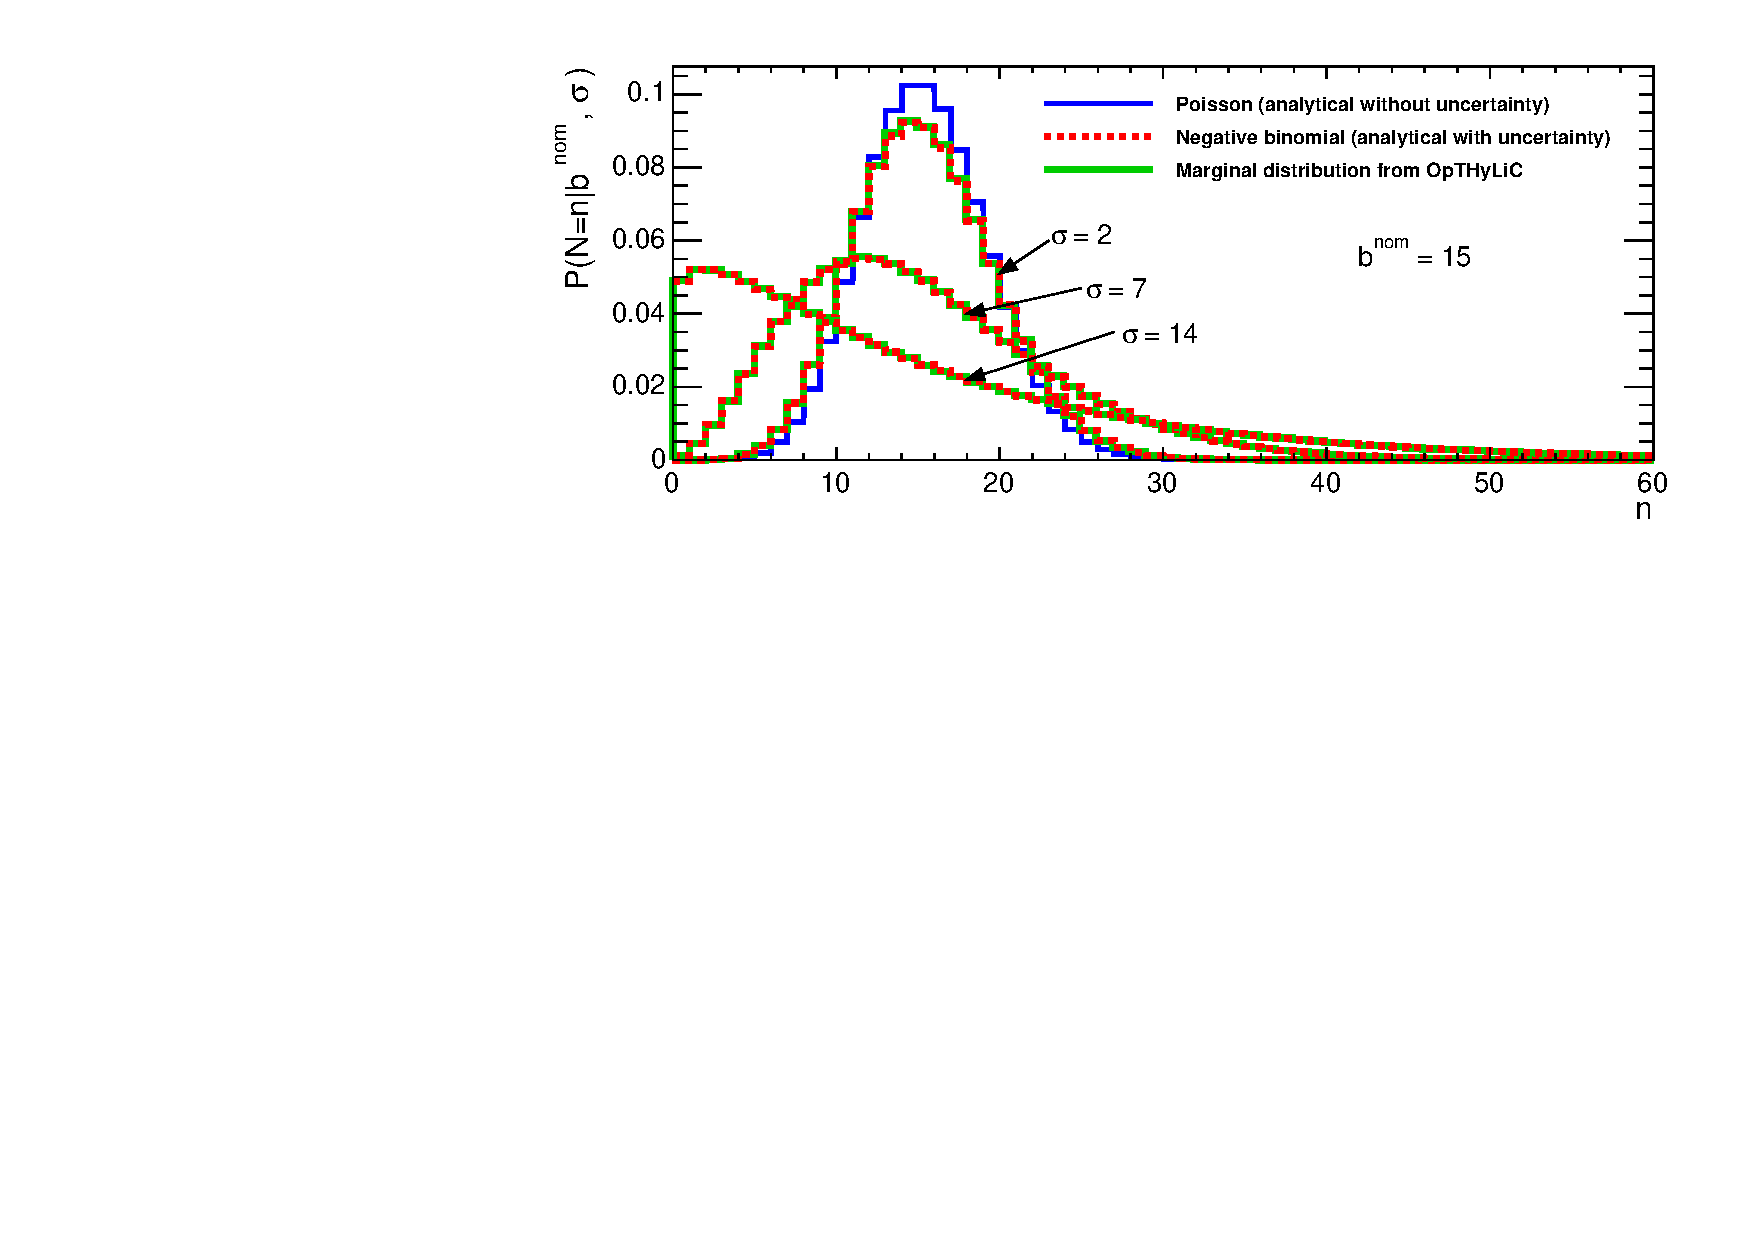
\includegraphics[width=1.2\textwidth]{Figures/Stat/SingleChannelStatUncertNegativeBinomial.pdf}\\
\pause
\vspace*{-0.9cm}
\hspace*{0.5cm}
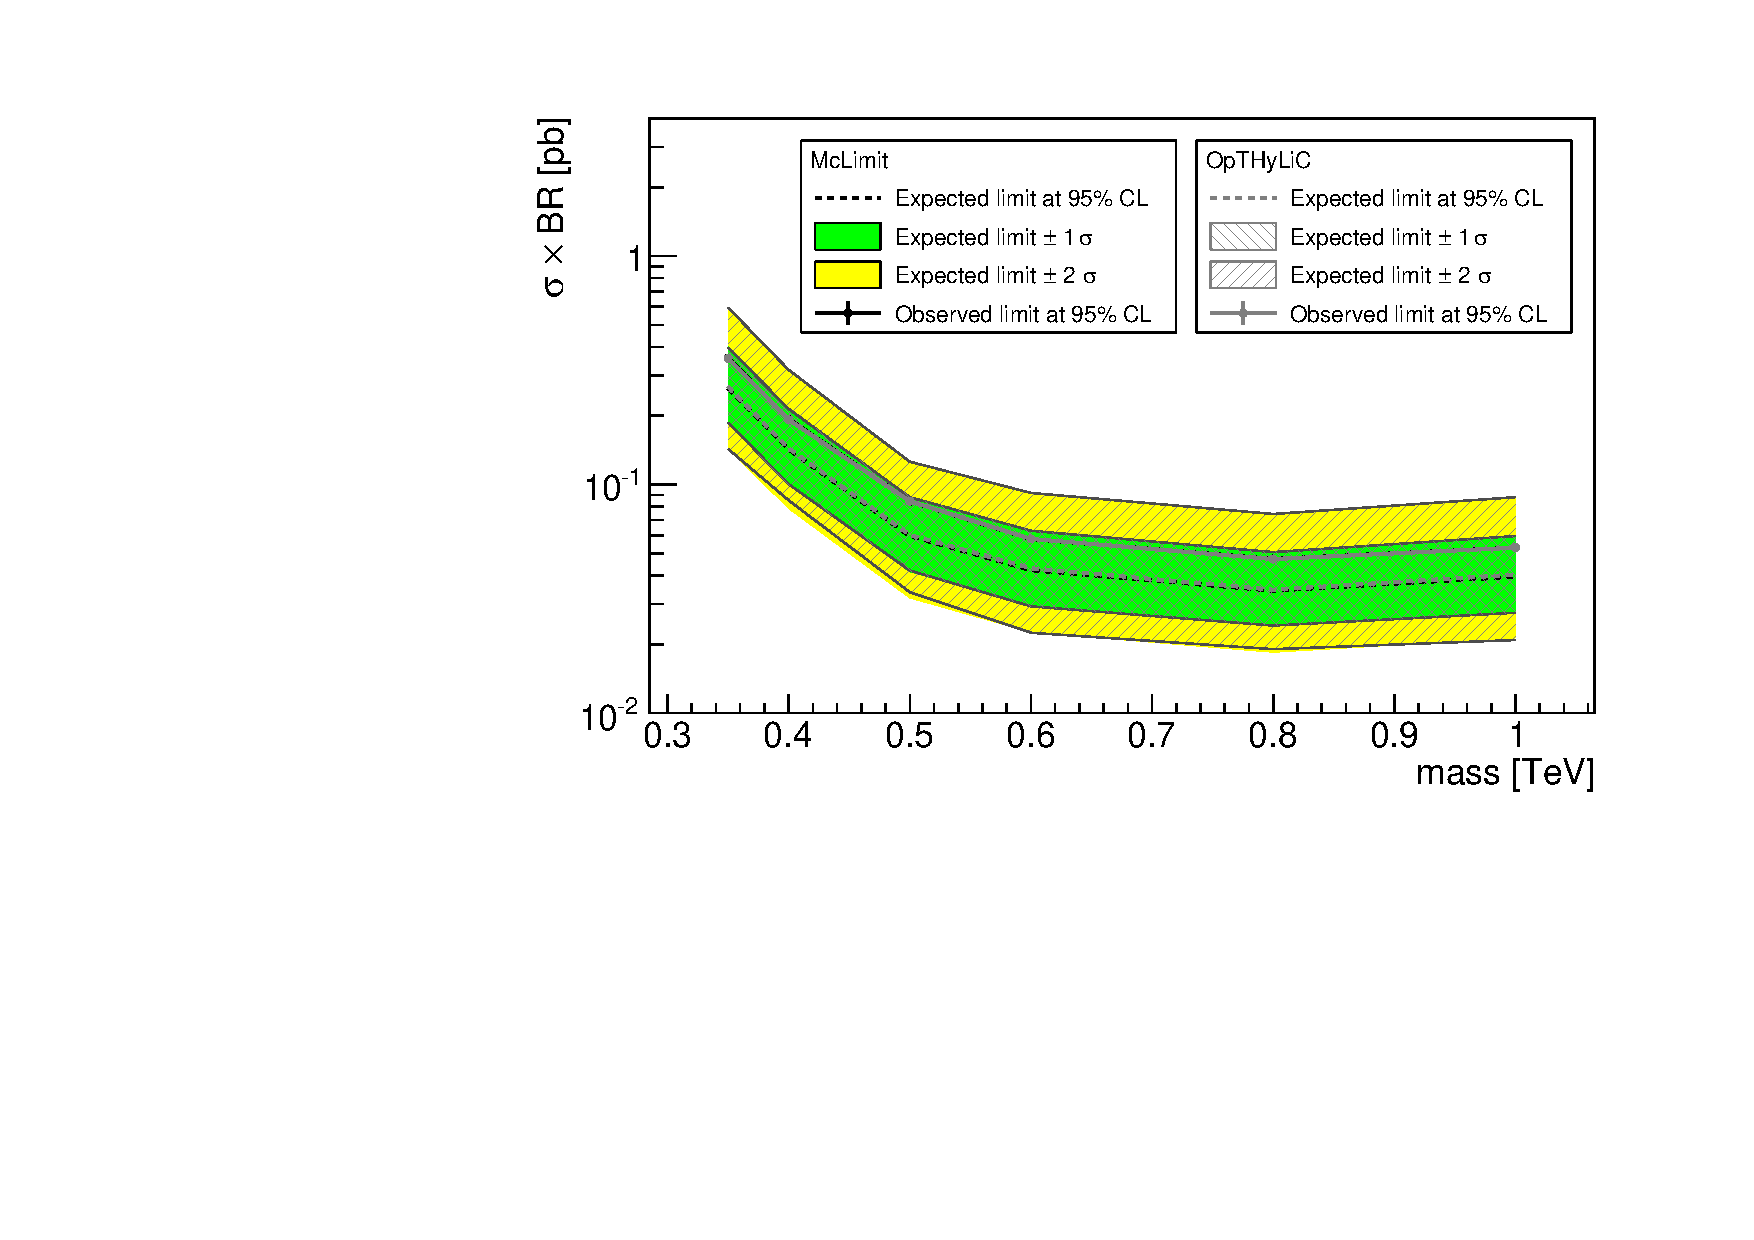
\includegraphics[width=1\textwidth]{Figures/Stat/ExclusionPlot_Sgluon.pdf}
%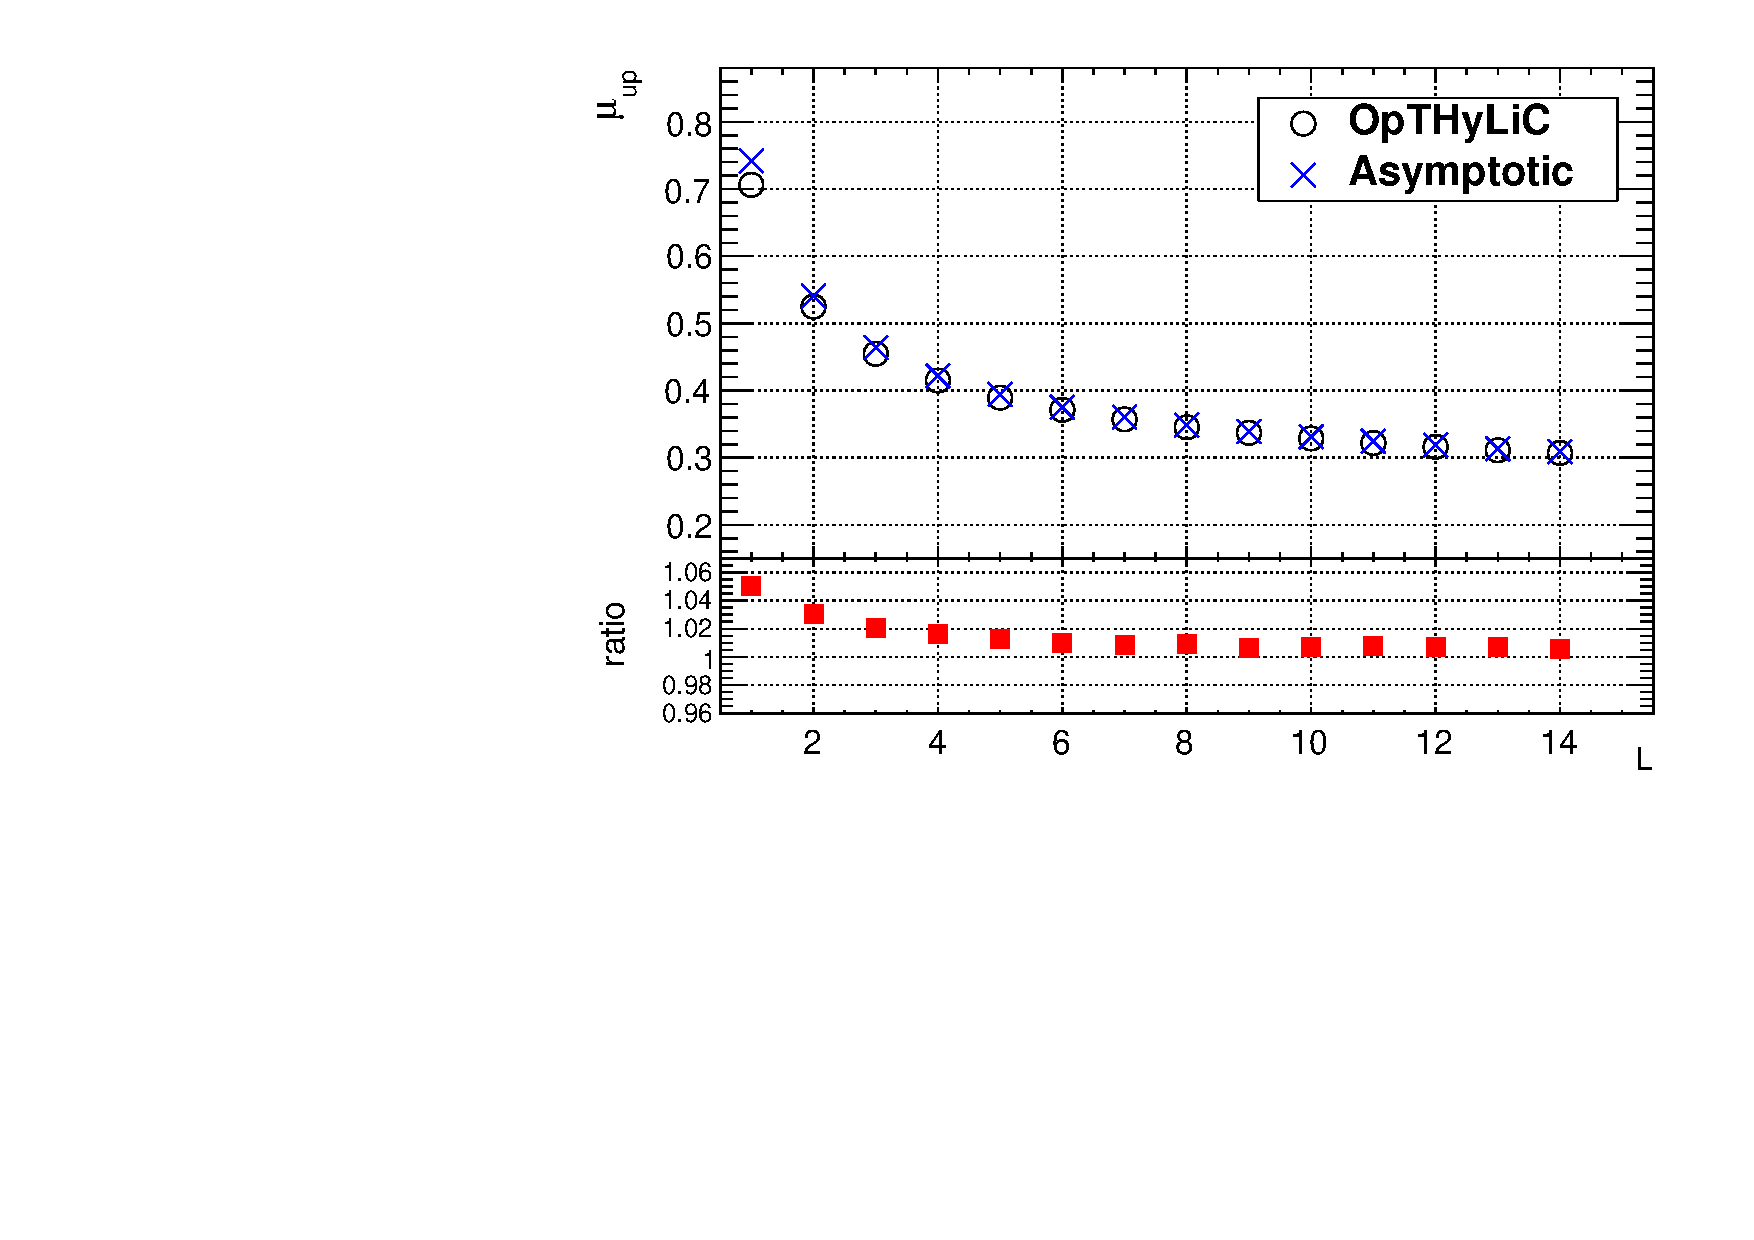
\includegraphics[width=0.48\textwidth]{Figures/Stat/MultipleChannelsNoUncertainties_OTHVsAsymptotic.pdf}
\end{center}
\end{figure}
\end{column}

\end{columns}
\end{frame}

\begin{frame}
\frametitle{\tifosi}

\vspace*{-0.8cm}
\begin{columns}
\begin{column}{0.5\textwidth}
\begin{block}{}
\begin{maliste}
\item Modèle statistique $\rightarrow$ \roofit
\begin{itemize}
\item Exactement le même que dans \OTH
\end{itemize}
\item Intégration \english{posterior} par chaîne de Markov $\rightarrow$ \roostats
%\begin{center}
%\hspace*{-0.5cm}
%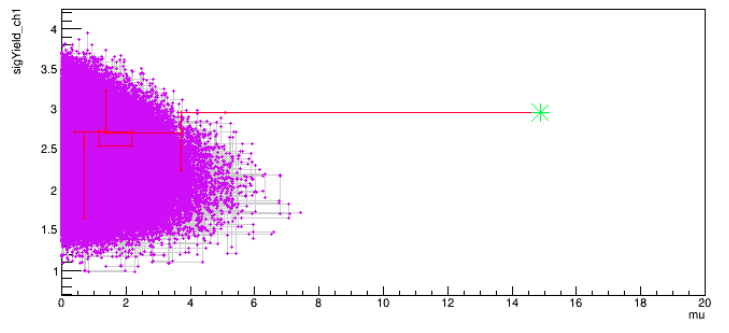
\includegraphics[width=0.90\textwidth]{Figures/Stat/MarkovChainIllustration.png}
%\end{center}
\item Validation : comparaison avec
\begin{itemize}
\item Solutions analytiques
\item \OTH
\end{itemize}
\end{maliste}
\end{block}
\end{column}

\begin{column}{0.5\textwidth}

\begin{center}
%\vspace*{-0.3cm}
%\hspace*{-0.9cm}
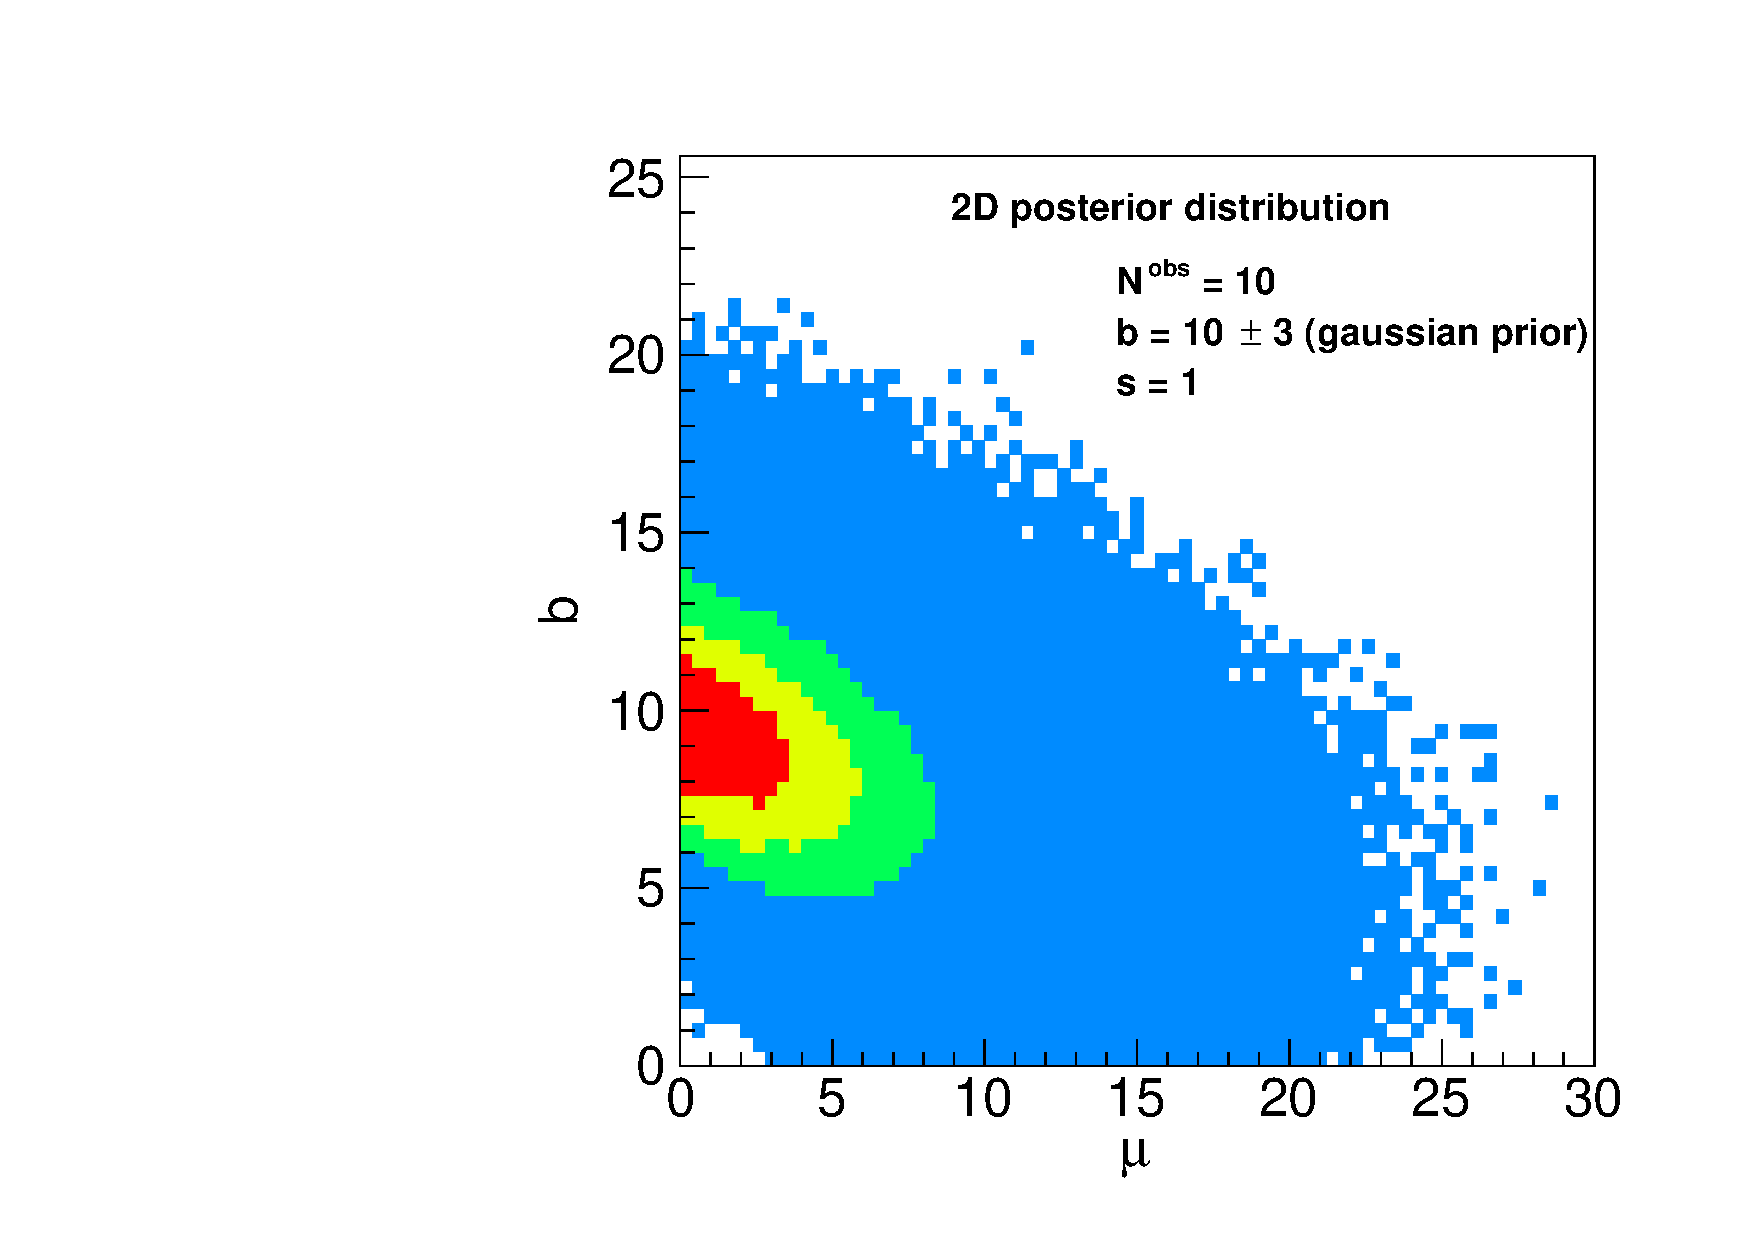
\includegraphics[width=0.55\textwidth]{Figures/Stat/Posterior2DPoissonWithUncertainBkg.pdf}
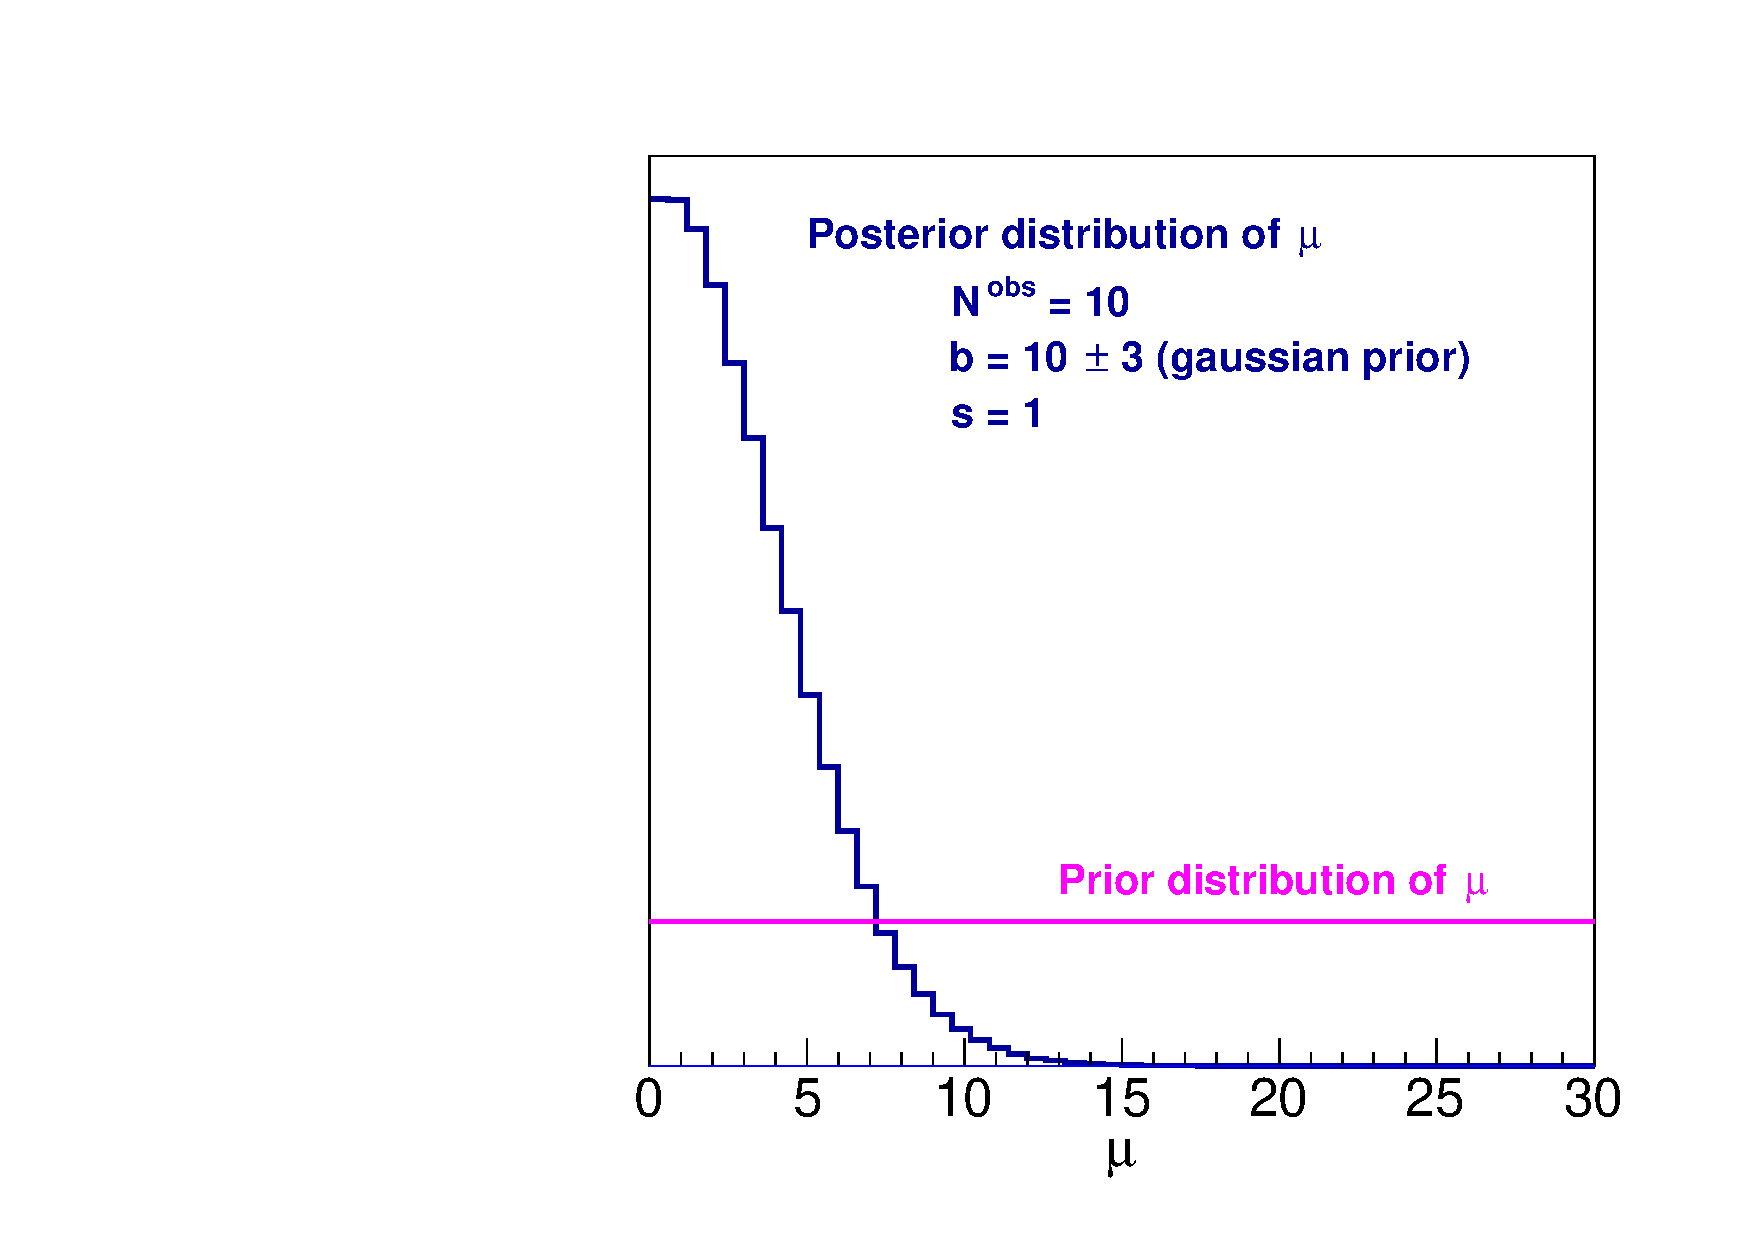
\includegraphics[width=0.55\textwidth]{Figures/Stat/PosteriorSignalPoissonWithUncertainBkg.pdf}
\end{center}

\pause

\begin{figure}[!htb]
\begin{center}
\vspace*{-1cm}
\hspace*{-0.3cm}
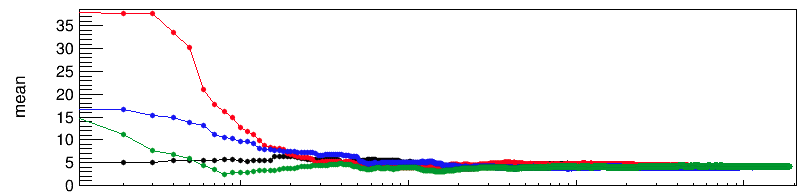
\includegraphics[width=1.1\textwidth]{Figures/Stat/cMu_cropped1.png}
\end{center}
\end{figure}

\end{column}
\end{columns}

\pause

\begin{figure}[!htb]
\begin{center}
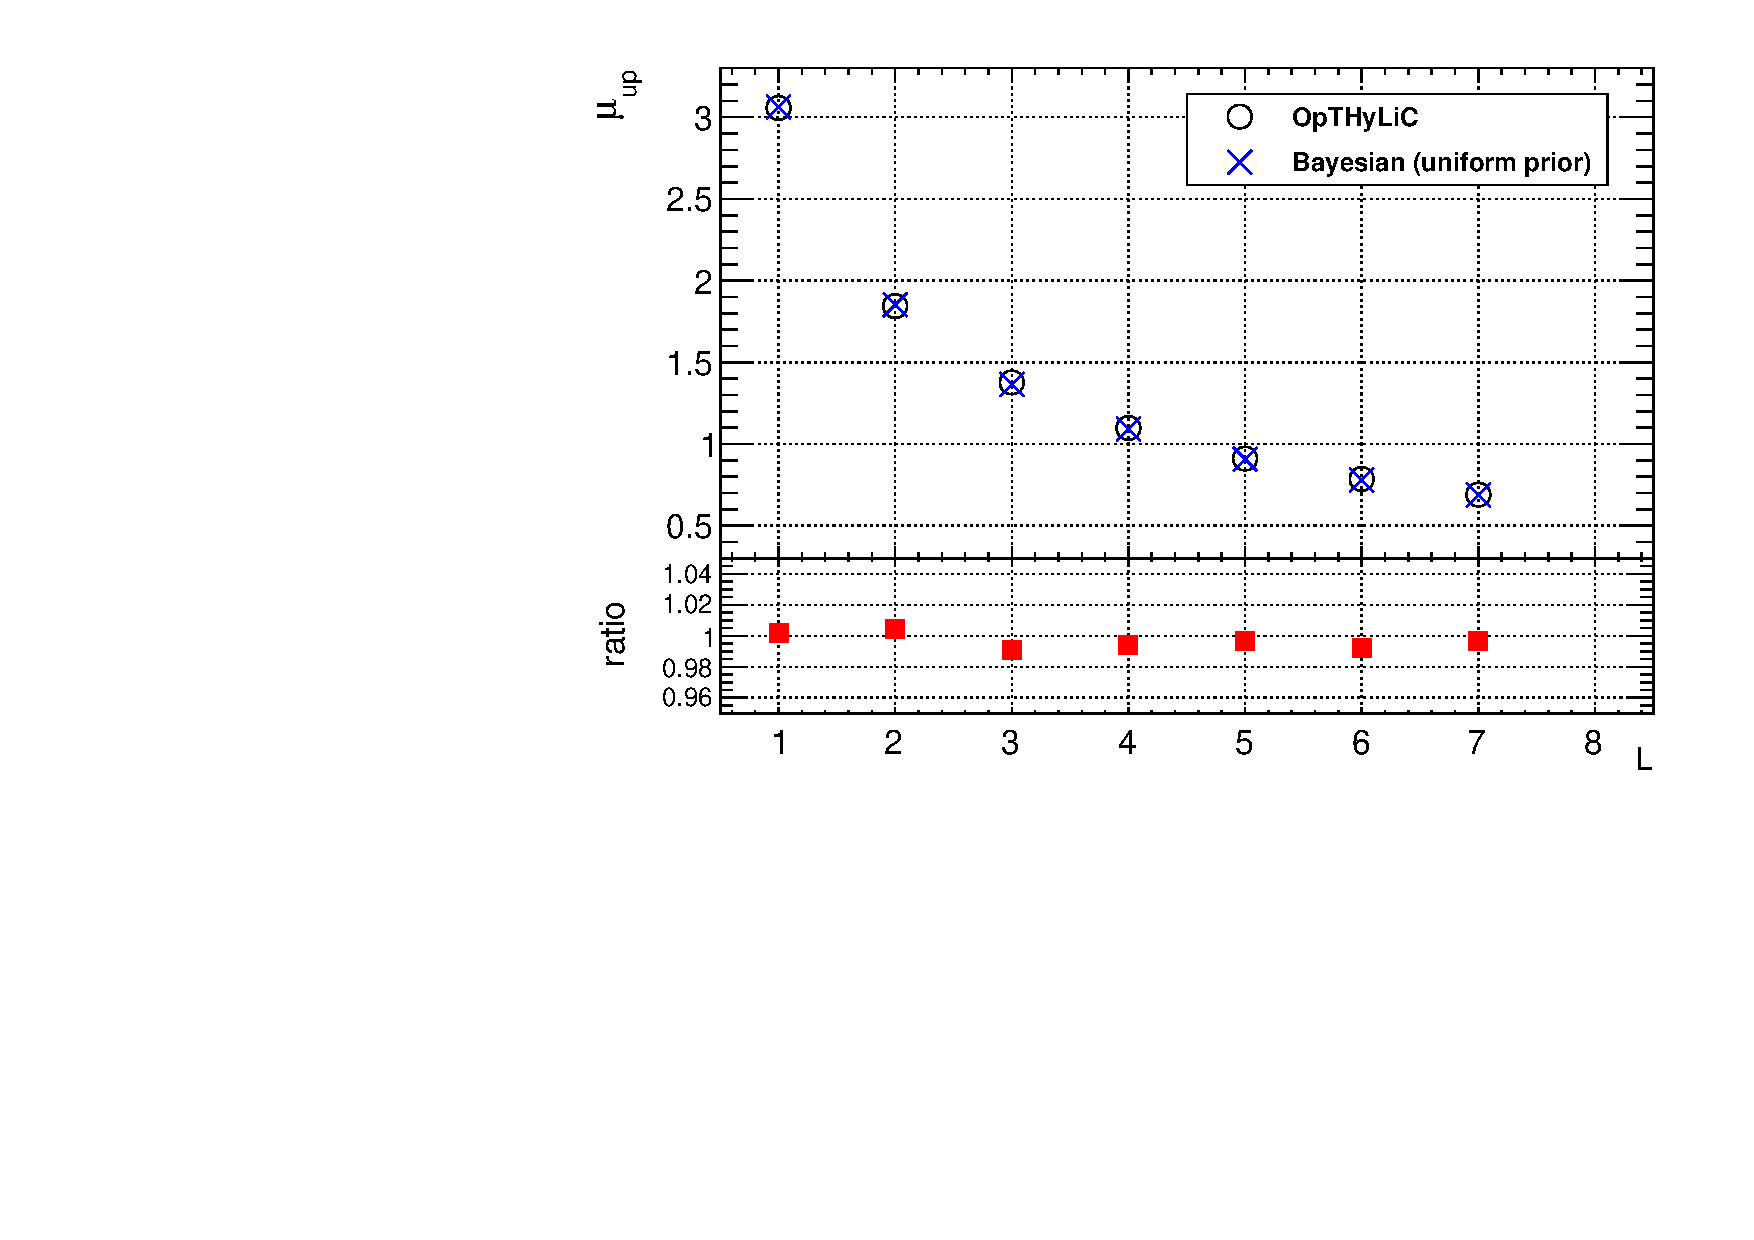
\includegraphics[width=0.5\textwidth]{Figures/Stat/SingleChannelForComparisonWithUncertaintiesOnBkg.pdf}
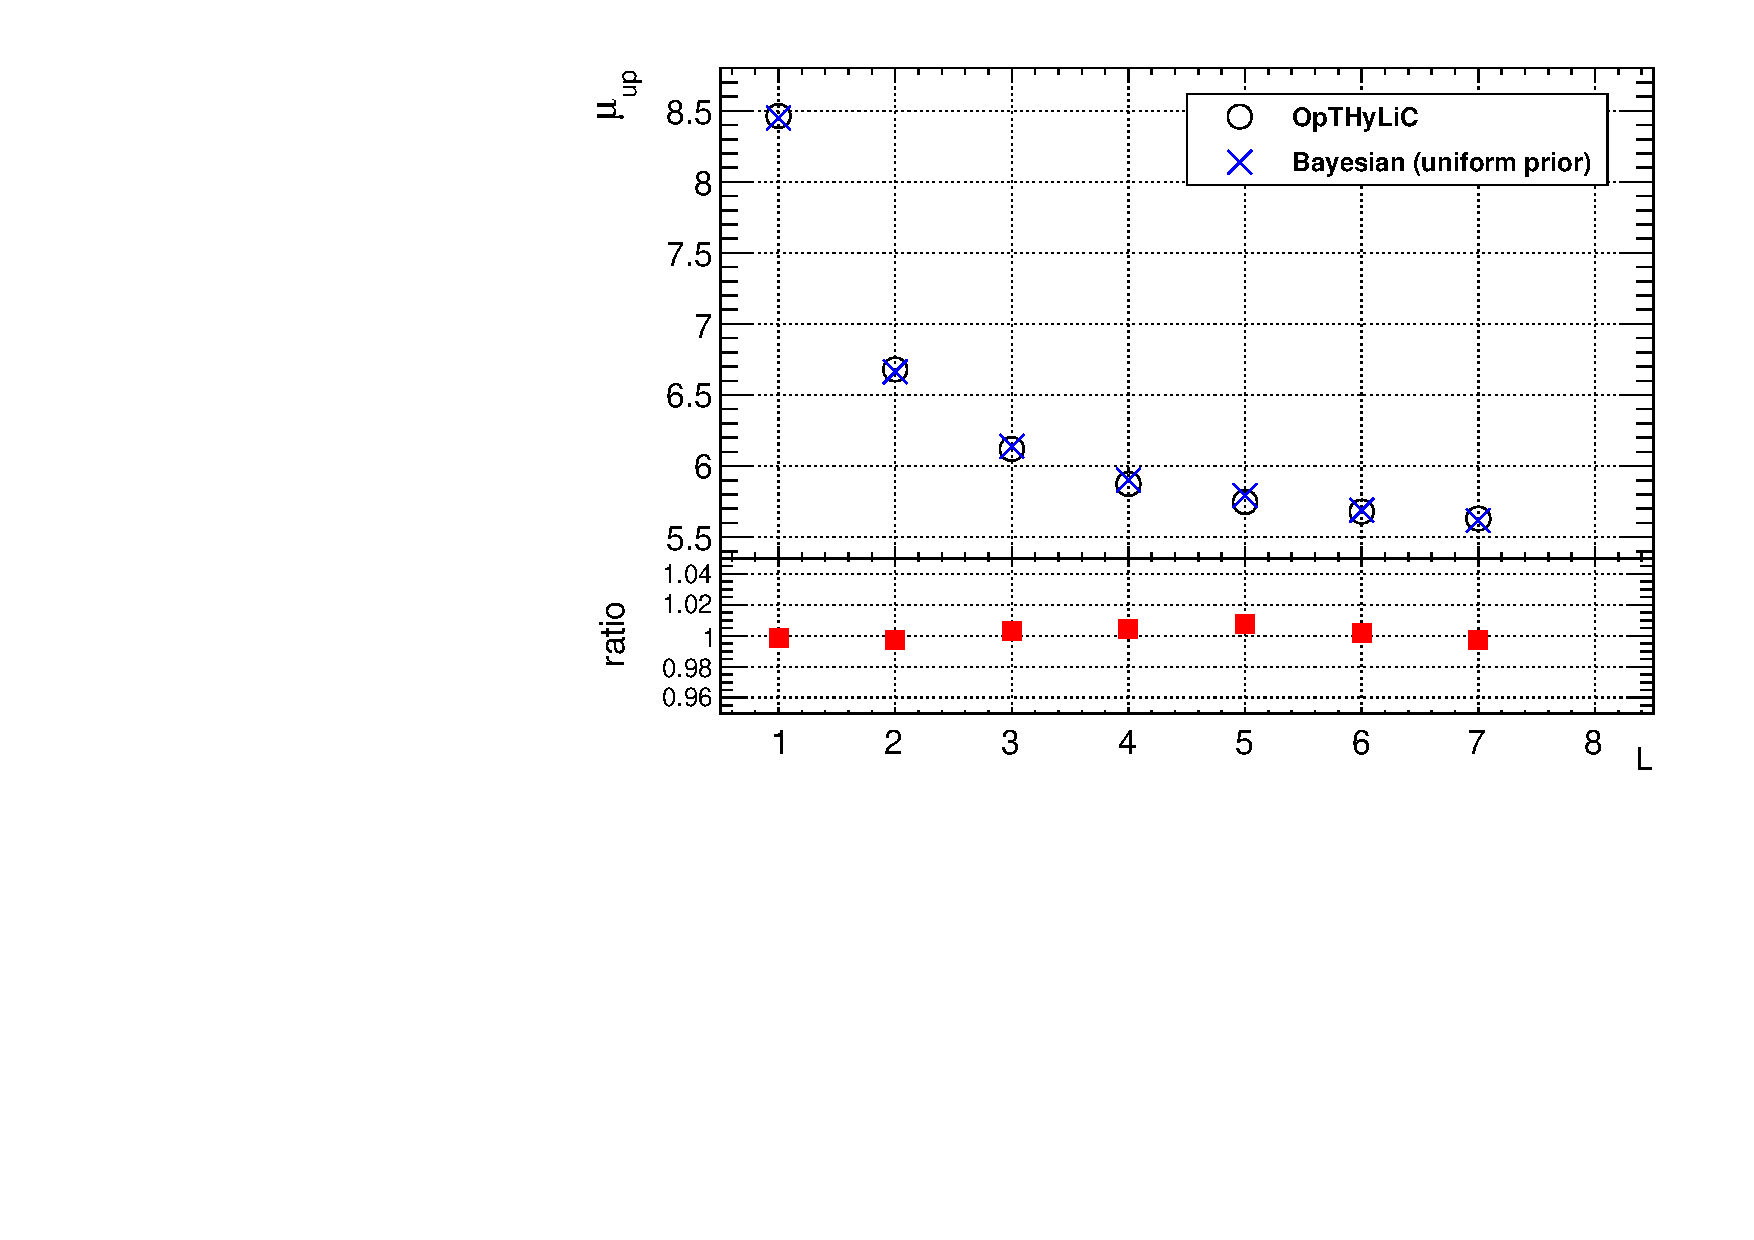
\includegraphics[width=0.5\textwidth]{Figures/Stat/SingleChannelWithUncertaintiesOnBkg.pdf}
\end{center}
\end{figure}

\end{frame}


